\documentclass{sigchi}

% Use this command to override the default ACM copyright statement (e.g. for preprints). 
% Consult the conference website for the camera-ready copyright statement.


%% EXAMPLE BEGIN -- HOW TO OVERRIDE THE DEFAULT COPYRIGHT STRIP -- (July 22, 2013 - Paul Baumann)
% \toappear{Permission to make digital or hard copies of all or part of this work for personal or classroom use is 	granted without fee provided that copies are not made or distributed for profit or commercial advantage and that copies bear this notice and the full citation on the first page. Copyrights for components of this work owned by others than ACM must be honored. Abstracting with credit is permitted. To copy otherwise, or republish, to post on servers or to redistribute to lists, requires prior specific permission and/or a fee. Request permissions from permissions@acm.org. \\
% {\emph{CHI'14}}, April 26--May 1, 2014, Toronto, Canada. \\
% Copyright \copyright~2014 ACM ISBN/14/04...\$15.00. \\
% DOI string from ACM form confirmation}
%% EXAMPLE END -- HOW TO OVERRIDE THE DEFAULT COPYRIGHT STRIP -- (July 22, 2013 - Paul Baumann)


% Arabic page numbers for submission. 
% Remove this line to eliminate page numbers for the camera ready copy
% \pagenumbering{arabic}


% Load basic packages
\usepackage{balance}  % to better equalize the last page
\usepackage{graphics} % for EPS, load graphicx instead
\usepackage{times}    % comment if you want LaTeX's default font
\usepackage{url}      % llt: nicely formatted URLs
\usepackage{makecell}
\usepackage{changepage}
\usepackage{mathtools}

% llt: Define a global style for URLs, rather that the default one
\makeatletter
\def\url@leostyle{%
  \@ifundefined{selectfont}{\def\UrlFont{\sf}}{\def\UrlFont{\small\bf\ttfamily}}}
\makeatother
\urlstyle{leo}


% To make various LaTeX processors do the right thing with page size.
\def\pprw{8.5in}
\def\pprh{11in}
\special{papersize=\pprw,\pprh}
\setlength{\paperwidth}{\pprw}
\setlength{\paperheight}{\pprh}
\setlength{\pdfpagewidth}{\pprw}
\setlength{\pdfpageheight}{\pprh}

% Make sure hyperref comes last of your loaded packages, 
% to give it a fighting chance of not being over-written, 
% since its job is to redefine many LaTeX commands.
\usepackage[pdftex]{hyperref}
\hypersetup{
pdftitle={SIGCHI Conference Proceedings Format},
pdfauthor={LaTeX},
pdfkeywords={SIGCHI, proceedings, archival format},
bookmarksnumbered,
pdfstartview={FitH},
colorlinks,
citecolor=black,
filecolor=black,
linkcolor=black,
urlcolor=black,
breaklinks=true,
}

% create a shortcut to typeset table headings
\newcommand\tabhead[1]{\small\textbf{#1}}


% End of preamble. Here it comes the document.
\begin{document}

\title{User-Defined Game Control with \\Smart Glasses in Public Space}

\author{\alignauthor Anonymous
\affaddr{Anonymous} \\ 
\email{Anonymous@Anonymous.Anonymous}
%\author{\alignauthor Chun-Yen Hsu, Ying-Chao Tung, Han-Yu Wang, \\Silvia Chyou, Jer-Wei Lin, Mike Y. Chen\\
%\affaddr{Mobile and HCI Research Lab, National Taiwan University} \\ 
%\email{\{hcythomas0125,tony61507,huw12313212,silvia.chyou,evin92\}@gmail.com,\\ mikechen@csie.ntu.edu.tw}
}


\maketitle




\begin{abstract}
Without specific game controller and direct-touch, game control on Smart Glasses differs with existing console and mobile games. Although current game control set on Smart Glasses is explored by developers based on system capability, the set is not reflective of user behavior.
To create better game control, we presented an user-defined game control study in public space to collect user behavior. In all, 2448 game control from 24 participants were logged, analyzed, and paired with think-aloud data for 17 commands performed with 3 interaction methods (On-Body, In-Air and Phone) and 2 glasses forms (Google Glass and Epson BT-100). 
Our findings indicate that users choose area relatively unobtrusive to perform the game control, and glasses form does influence how users creates game control. We also present a complete user-defined game control set with agreement scores and taxonomy. 
Our results will help designers create better game control sets informed by user behavior.
\end{abstract}


\keywords{
  Game, input, control, smart glasses, guessability, think-aloud, user-defined, public space, pervasive gaming, wearable.
	% Guides; instructions; author's kit; conference publications;
	% keywords should be separated by a semi-colon. \newline
	% \textcolor{red}{Optional section to be included in your final version, 
 %  but strongly encouraged.}
}

\category{H.5.2.}{Information Interfaces and Presentation}
: User Interfaces - \emph{Interaction styles, evaluation/methodology, user-centered design.}
% See: \url{http://www.acm.org/about/class/1998/}
% for more information and the full list of ACM classifiers
% and descriptors. \newline
% \textcolor{red}{Optional section to be included in your final version, 
% but strongly encouraged. On the submission page only the classifiers’ 
% letter-number combination will need to be entered.}



\section{Introduction}

 \begin{figure}[!h]
  \centering
  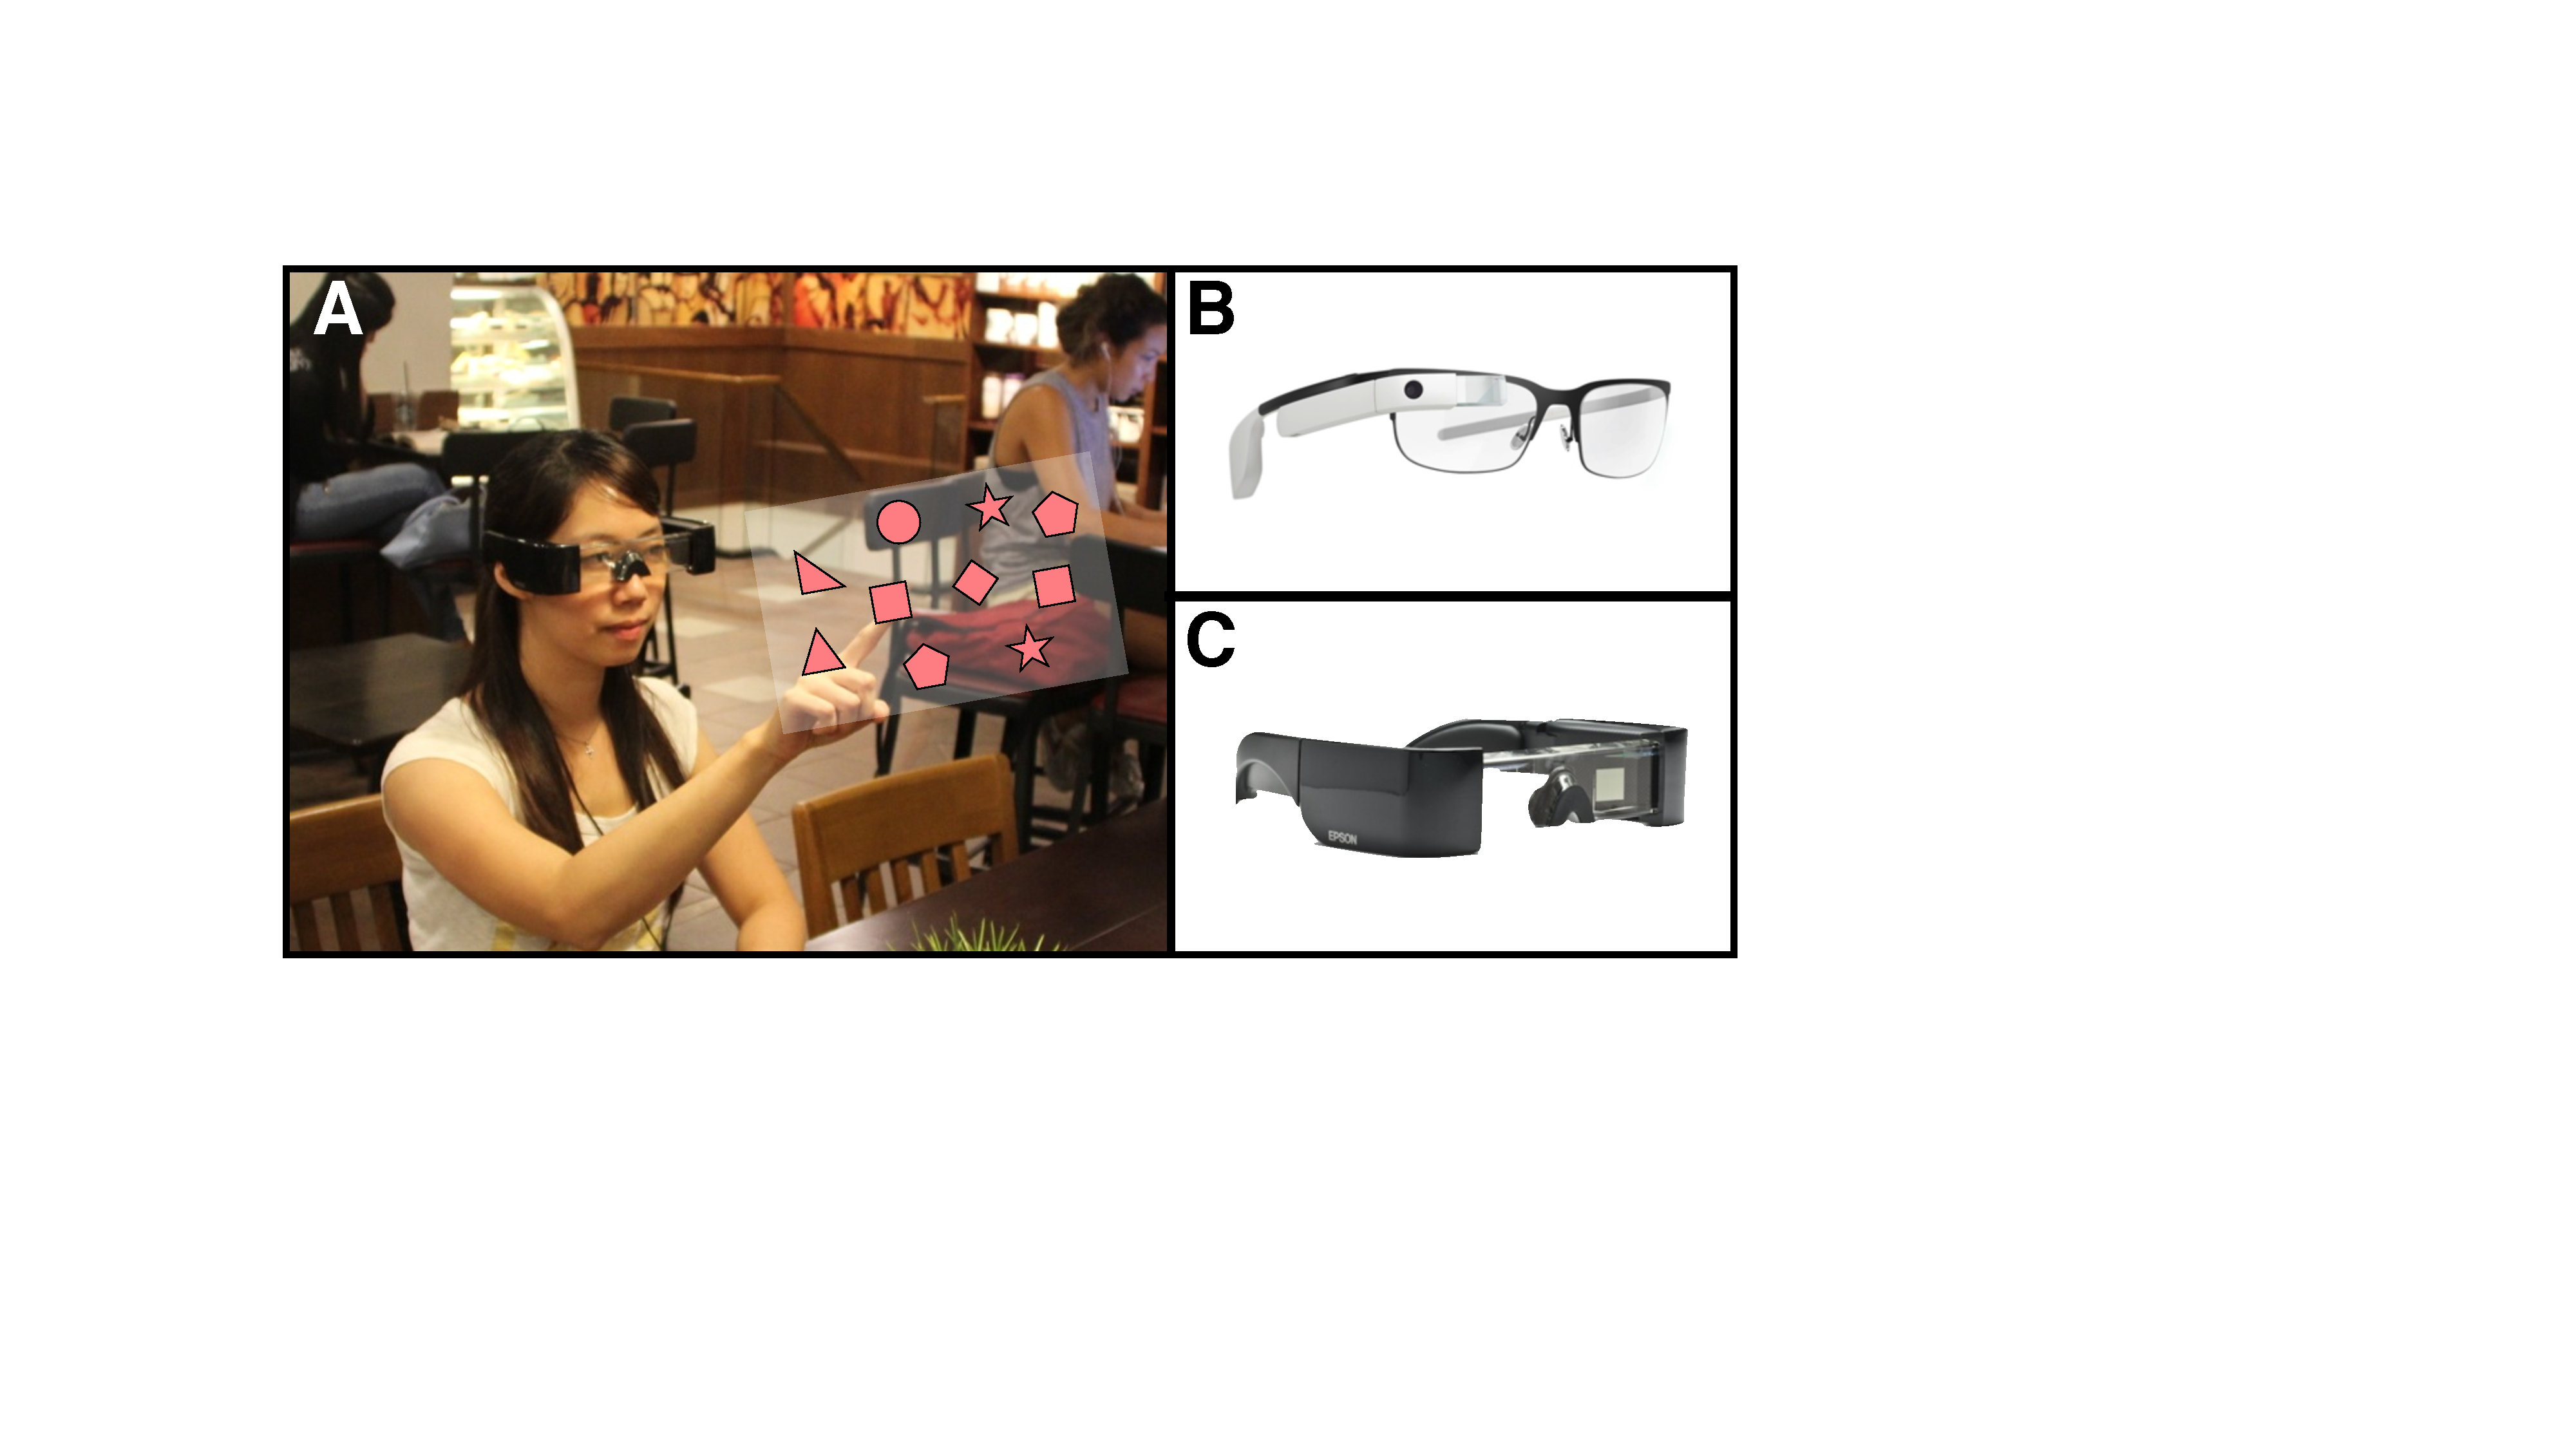
\includegraphics[width=1\columnwidth]{TopFigure.pdf}
  \caption{In a Starbuck cafe, a user performing a in-air gesture to select a single object after being prompted by an animation demonstrating the selecting effect (a pop out animation).}
  \label{fig:TopFigure}
  \end{figure} 

%The invention of smart glasses offers more 
%Emerging wearable computing devices atrract extensive attention worldwide. 
Samrt Glasses offer the opportunity to achieve always available gaming and play instantly. We can play a game without any setup. Smart glasses, such as Google Glass and Epson BT-100 Smart Glasses, are computerized eyeglasses and are usually equipped with various sensors, such as camera, gyroscope, accelerometer and GPS, to enrich their capabilities. 
Without specific game controller and touch-screen, game control on Smart Glasses differs with existing consoles and mobile games. There is no general game control set existed nowadays for smart glasses gaming. However, Some developers explored several game control sets based on system capacitlity. Take mini games \cite{MiniGames} provided by Google for example, ``Balance'' uses gyroscope to capture head gesture as game input. With built-in microphone,``Clay Shooter'' utilizes voice to trigger gun fire, and ``Shape Spitter'' uses in-air gesture in front of their camera.  
Nevertheless, what kinds of control actions do regular users make? In users' minds, what charateristics are important for such game controls? Will they choose direct-touch-like control or just a controller usage? How consistent are game controls employed by different users for the same game task? 
Although designers may organize their game controls in a principled, logical fashion, user behavior is rarely so systematic. As McNeill \cite{HandAndMind} writes in his laborious study of human discursive gesture, ``Indeed, the important thing about gestures is that they are \emph{not} fixed. They are free and reveal the idiosyncratic imagery of thought''.

To investigate these idiosyncrasies, we employ a guessability study methodology \cite{Wobbrock:2005:MGS:1056808.1057043} that presents the \emph{effects} of game controls to participants and elicits the \emph{causes} meant to invoke them in a real-world environment. By interview and video analysis, we obtain rich qualitative data that illuminates users' mental models. By collecting preference score with different interaction methods and glasses forms, we obtain a significant difference between different interaction methods. And we find glasses form does influence on how user creates game controls. The final result is a detailed picture of user-defined game controls and the mental models that accompany them. Although some prior works explored smart glasses inputs \cite{Colaco:2013:MCL:2501988.2502042,Serrano:2014:EUH:2611247.2556984}, our work is the first one to utilize users, rather than principles, in the development of a glass gaming control set. Moreover, we explicitly recruited regular people without prior experience using smart glasses (e.g. the Google Glass or Epson BT-100) expecting that they would behave with and reason about interactive smart glasses differently than designers and system builders.

This work contributes the following to glass gaming resarch: 
(1) a quantitative and qualitative characterization of user-defined game controls, including a taxonomy, 
(2) a user-defined game control set, 
(3) insight into users' mental models when making game controls in public space with understanding of implications for mobile-input technology. 
Our results will help designers create better game controls informed by user behavior.


% and were interviewed about the control detail
%To reflective of user behavior.
%Although current game control set on Smart Glasses is explored by capability 

%A. Review現有遊戲平台及操作方式。
%B. Smart Glass帶來新的可能性,跟傳統遊戲的區別。 
%C. 現有的Smart Glass Gaming有哪些,而且目前體驗很差。
%D. 我們認為造成體驗差的原因,跟我們的解法。


\section{Related Work}

    \subsection{Game Control}
    There are two main research fields related to game controls. One is comparing existing game controls with player expereience. For examples, Cairns et al.\cite{Cairns:2014:ICI:2556288.2557345} looked at how the naturalness of the game controls influences the experience of immersion in mobile games; The study of Birk et al.\cite{Birk:2013:CYG:2470654.2470752} showed that there were a number of controller effects on player experience and in-game player personality; Lankes et al.\cite{Lankes:2012:CVC:2367616.2367629} investigated the relationship between the feeling of being in control in a game situation and the interaction complexity; Park et al.\cite{Park:2014:HFS:2556288.2557091} examined the characteristics of a speed-based exergame controller that bear on human factors; Cheema et al.\cite{Cheema:2011:WWT:2159365.2159407} explored aspects of players experience in first person games that use 3D gestures for interaction.

    Another field is to explore new kind of game control inputs. Previous works\cite{Ekman:2008:IEU:1358628.1358820,Vickers:2013:PLT:2531922.2514856,Sundstedt:2010:GGU:1837101.1837106,Smith:2006:UEM:1178823.1178847} shows the possibility to use eye gesture as game inputs; Christian et al.\cite{Christian:2014:VSI:2559206.2580103} and Yim et al.\cite{Yim:2008:EDD:1496984.1497033} provided novel techniques for users to interact with games by head-gesture; Harada et al.\cite{Harada:2011:VGI:2042053.2042059} and Sporka et al. \cite{Sporka:2006:NIS:1168987.1169023} both indicated that the voice input greatly expanded the scope of games that could played with hands-free and just counted on voice; Baba et al.\cite{Baba:2007:VGU:1278280.1278285} presented a game prototype which treated skin contact as controller input; Nacke et al.\cite{Nacke:2011:BGD:1978942.1978958} so far as to considered using biofeedback (including EMG, EDA, EKG, RESP, TEMP) as game input methods.


    \subsection{Mobile Input Technology}
    Some works related to mobile systems had defined designer-made control methods. These systems could be divided into two main categories, in-air gestures and on-body inputs. Kim et al.\cite{Kim:2012:DFI:2380116.2380139} developed a wrist-worn architecture, which supports discrete gesture recognition with reconstructing a 3D hand model in the air. Similarly, Jing et al.\cite{Jing:2013:MRS:2541831.2541875} implemented \textsl{Magic Ring}, a finger ring shaped input device using inertial sensors to detect subtle finger gestures; Cola\c{c}o et al.\cite{Colaco:2013:MCL:2501988.2502042} built a head-mounted display, \textsl{Mime}, sensing 3D gestures in front of users' eyes. 

    Harrison et al.\cite{Harrison:2011:OWM:2047196.2047255} created \textsl{OmniTouch}, a wearable depth-sensing and projected system that enables interactive multitouch applications on any surface of users' body. Moreover, \textsl{Skinput}\cite{Harrison:2010:SAB:1753326.1753394}, a technology that appropriates the human body for acoustic transmission, and allows the skin to be used as an input surface. Baudisch al.\cite{Gustafson:2011:IPL:2047196.2047233} illustrated a concept of imaginary interface with sensing several gestures on users' palms. Recently, Serrano et al.\cite{Serrano:2014:EUH:2611247.2556984} explored the use of \textsl{Hand-to-Face} input to interact with head-worn displays(HWD) and provided a set of guidlines for developing effective Hand-to-Face interactions based on two main facotrs they found, social acceptability and cultural effect.

    \subsection{User Elicitation Studies}
    User-elicitation studies are a specific type of participatory design methodology that involves end-users in the design of gesture-sets\cite{Good:1984:BUI:358274.358284,Morris:2012:WWI:2396636.2396651}. These studies had been used to design user interfaces of various types including multi-touch gestures on small and large surfaces\cite{Anthony:2012:IRC:2396636.2396671,Epps:2006:SHS:1125451.1125601,Wobbrock:2009:UGS:1518701.1518866,Findlater:2012:BQA:2207676.2208660} and multi-modal interactions \cite{Morris:2012:WWI:2396636.2396651,Valdes:2014:EDS:2611222.2557373}. There is also some evidences that user-defined control sets are more complete than those sets defined solely by experts\cite{Anthony:2012:IRC:2396636.2396671,Pyryeskin:2012:CEG:2396636.2396638,Wobbrock:2009:UGS:1518701.1518866}.

    In a user-elicitation study, users were shown referents (an action’s effects) and were asked to demonstrate the interactions that resulted in a given referent\cite{Wobbrock:2009:UGS:1518701.1518866}. In this work, we draw upon the user-elicitation methodology to identify user expectations and suggestions for smart glass gaming.

\section{Developing a User-Defined Game Control Set}
%需要描述場域嘛?


    \subsection {Overview and Rationale}
    Playing game is a \textsl{user-computer dialogue}\cite{userComputer}, a conversation mediated by language of inputs and outputs. As in any dialogue, feedback is essential to conducting this conversation. When something is misunderstood between humans, it may be rephrased. The same is true for user-computer dialogues. Feedback, or lack thereof, either endorses or deters a player's action, causing the player to revise his or her mental model and possibly take a new action.

    In developing a user-defined game control set, we did not want the limitation of input technology to influence users' behavior. Hence, we sought to remove the \textsl{gulf of execution}\cite{gulf} from the dialogue, creating, in seence, a monologue in which the player's behavior is always acceptable. This enables us to observe users' unrevised behavior, and drive system design to accommodate it.

    In view of this, we developed a user-defined game control set by having 24  participants perform game control with 2 Smart Glasses (Google Glass and Epson BT-100) in a public cafe. To avoid bias from visual hint\cite{Epps:2006:SHS:1125451.1125601}, no elements specific to Mobile, Console, PC games were shown. Similarly, no specific game title was assumed. Instead, participants acted in a simple blocks world of geometry shapes or basic human avatar. Each participant saw the effect of a game control (e.g., an object moving left and right) and was asked to perform the game control he or she thought would cause that effect (e.g. moving the finger tip left and right in front of their chest). In another word, the effect of a game control is the \textsl{game task} to which the game control try to complete.

    Seven-teen game tasks were presented, and game controls were elicited for three different interaction methods (\emph{In-Air}, \emph{On-Body}, \emph{Phone}). The system did not attempt to sense the users' control input, but we use a camera to record the whole control process. Participants used the think-aloud protocol and were interviewed about the control detail. They also supplied subjective preference ratings.

    The final user-defined game control set was developed in light of the \textsl{agreement} participants exhibited in choosing control action for each game task\cite{Wobbrock:2005:MGS:1056808.1057043}. The more participants that used the same action for a given task, the more likely that control action would be assigned to that task. In the end, our user-defined game control set emerged as a surprisingly consistent collection founded on actual user behavior.
    %這邊要研究一下......why "surprisingly consistent"


    \subsection {Game Tasks}

    Casual game is one of the game categories with most players\cite{esa_ef_2014}, and it is shown high potential in public gaming\cite{Jurgelionis:2011:PET:2027456.2027462,Reis:2012:EMC:2405577.2405651,Biskupski:2014:DEB:2559206.2580097}. We choosed top 90 casual games\cite{TopGames} from existing platforms, including PCs, consoles and mobile games (30 games for each) by crawling and analyzing the sale and download count data from famous gaming websites\cite{appannie,VGChartz,Steam,GameStop}. We invited 3 experienced game developers to review these top 90 casual games. They found out 26 game tasks in total, and removed 9 tasks which were only used once in specific games. At last, we got a set of general casual game task(shown in Table \ref{tab:table1}) with 17 tasks, which can completely support 90\% of our top casual games. 

  \begin{table}
    \centering
    \begin{tabular}{|c|l|l|}
      \hline
      \tabhead{\#} &
      \multicolumn{1}{|p{0.4\columnwidth}|}{\centering\tabhead{Task}} &
      \multicolumn{1}{|p{0.45\columnwidth}|}{\centering\tabhead{Used in Famous Game}} \\
      \hline
      1 & Select Single & Clash of Clans, Plague Inc.\\
      \hline
      2 & Vertical menu & Puzzle\&Dragon, PeggleHD \\
      \hline
      3 & Horizontal menu & Clash of Clans, PeggleHD\\
      \hline
      4 & Move left and right & Temple Run, Super Mario\\
      \hline
      5 & Move in 4 directions & 1943, RaidenX\\
      \hline
      6 & Switch 2 objects & Candy Crush, Bejeweled\\
      \hline
      7 & Move object to position & World of Goo, The Sim\\
      \hline
      8 & Draw a path & Draw Something, P\&D\\
      \hline
      9 & Throw an object (in-2D) & Angry Birds, PeggleHD\\
      \hline
      10 & Note highway & RockSmith, Deemo\\
      \hline
      11 & Rotate an object (Z-axis) & Zuma, PeggleHD \\
      \hline
      12 & Rotate an object (Y-axis) & Spore, The Sim\\
      \hline
      13 & Avatar jump & Temple Run, Super Mario\\
      \hline
      14 & Avatar 3D move & Spore, Tintin\\
      \hline
      15 & Avatar attack & Minecraft, Terraria\\
      \hline
      16 & Avatar squat & Temple Run, Minecraft\\
      \hline
      17 & Viewport control & The Sim, Spore\\
      \hline

    \end{tabular}
    \caption{Summary of our general casual game task set. We named several famous games which uses these tasks.}
    \label{tab:table1}
  \end{table}


  \subsection {Participants}
  We recruited twenty-four participants from the mass population with equal sex ratio for our study. Their average age are 23.2 (\textsl{sd} = 2.72). All participants are right-handed and none of them had past experience with Smart Glasses usage. About their gaming experience, according to our investigation, 14 users were daily game players, 9 were weekly and 1 was monthly. Participants spent 1.36 hours (\textsl{sd} = 0.89) in average to play games one time. Moreover, 58\% of them indicated that their main gaming platforms were on mobile phones, 38\% were on PCs, and only 4\% were on consoles. Another important factor of gaming experience is the familiarity of game controllers. The result showed that, compared with joysticks, most of them were more familiar with keyboards, mouses and touch screens (see Figure~\ref{fig:figureFamiliarity}).
  %\begin{figure}[!h]
  %\centering
  %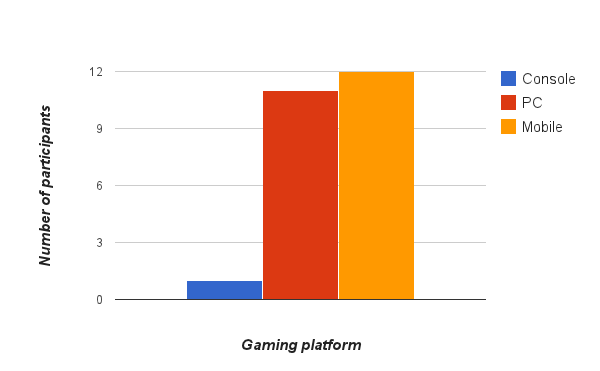
\includegraphics[width=0.9\columnwidth]{Platform}
  %\caption{With Caption Below, be sure to have a good resolution image
  %  (see item D within the preparation instructions).}
  %\label{fig:figurePlatform}
  %\end{figure} 
  %\begin{figure}[!h]
  %\centering
  %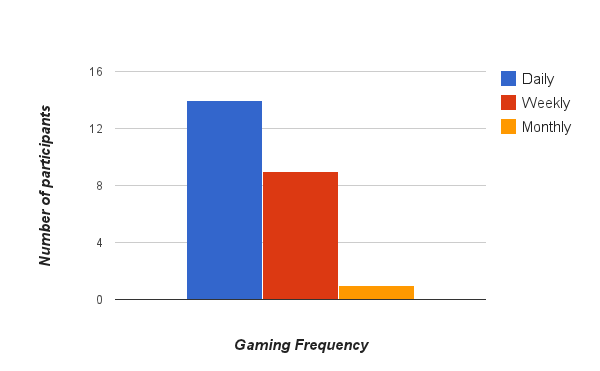
\includegraphics[width=0.9\columnwidth]{Frequency}
  %\caption{With Caption Below, be sure to have a good resolution image
  %  (see item D within the preparation instructions).}
  %\label{fig:figureFrequency}
  %\end{figure}
  \begin{figure}[!h]
  \centering
  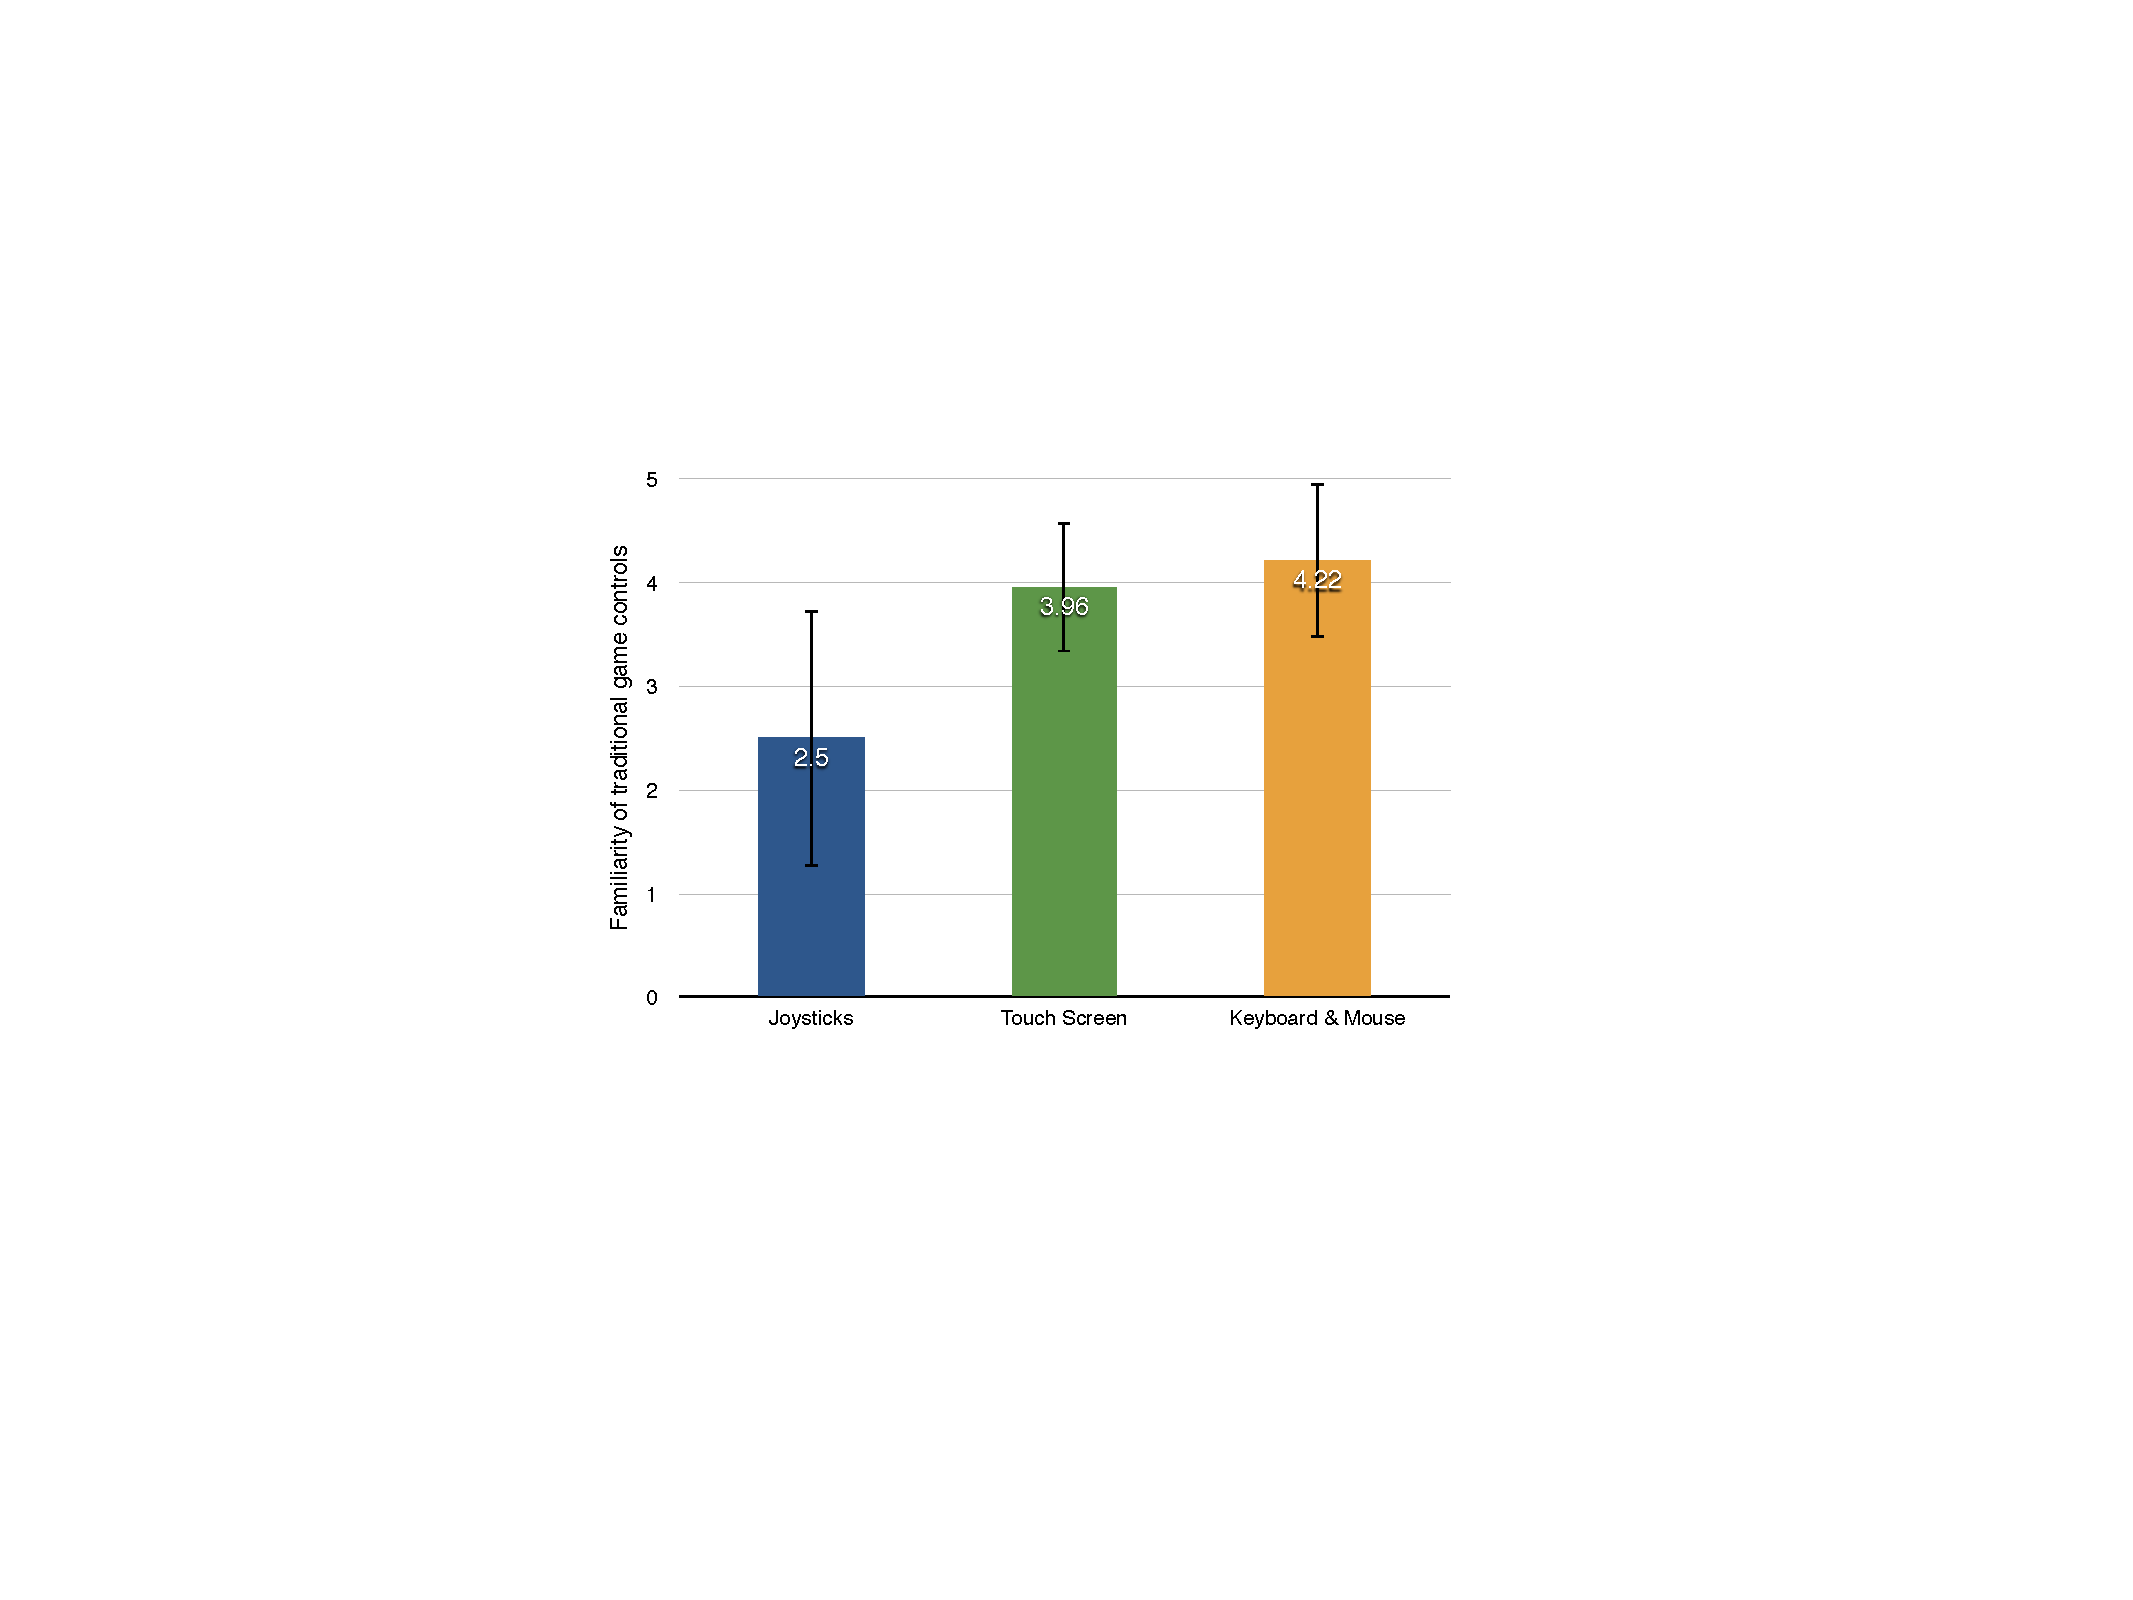
\includegraphics[width=1\columnwidth]{Familiarity.pdf}
  \caption{Users' game control familiarity.}
  \label{fig:figureFamiliarity}
  \end{figure}   

  \subsection {Field}
  According to the previous works\cite{Wiliamson:2011:MMI:2070481.2070551,Williamson:2013:MEM:2522848.2522874,Montero:2010:YUS:1851600.1851647,Rico:2010:UGM:1753326.1753458}, the social acceptability of a mobile-input was influenced by whether participants believed a bystander could interpret the intention of the control action. Therefore, to provide a game control set suited for a real world environment, we chose a Starbuck cafe near our college. The visitor flow of the cafe, averagely, was 72.5 people per hour. In our investigation, participants indicated that the cafe was comparatively a public space with average 4.17 points (\textsl{sd}=0.65) in a 5-point Likert Scale about degree of field publicity (1 means very private, 5 means very public).    

  \subsection {Glass Forms}
  There are many Smart Glasses with different screen sizes and screen placement on the current market. To observe the effect of distinct display designs upon the study result, our study conducted on two famous Smart Glasses, Epson BT-100 and Google Glass. The display of Epson BT-100 is located in front of the user's eyes with $960 \times 540$ resolution (equivalent of a 320" screen from 20 m away)\cite{BT100}. And Google Glass locates its display above the user's right eye with $640 \times 360$ resolution (equivalent of a 25" screen from 2.4 m away)\cite{GoogleGlass}.       

    \subsection {Interaction Methods}
    In our study, we asked users to define three control manners to satisfy three interaction requirements individually in each task. These three interaciton types, classified according to familiar interactions explored by previous works, were \textsl{In-Air}, \textsl{On-Body}, and \textsl{Phone}. \textsl{In-Air}, one of these types, was that users were asked to define a input method without touching any tangible object, such as, moving eyeballs, rotating their heads, voice control or in-air gestures. Another method was \textsl{On-Body}, which asked users to design a control action with touching any skin or accessories on their own bodies. The last method, \textsl{Phone}, was required users to create a game control by interacting with common always-available devices, mobile phones.    


    \subsection {Procedure}
    Users wore two different glasses (Epson BT-100 and Google Glass) and our software randomly presented 17 game tasks (Table \ref{tab:table1}) to participants. For each game task, participants performed a game control in 3 different interaction methods(in-air gesture, on-body input and phone interaction). And study conducted with a counterbalanced measures design with Glasses form and interaction method. After each game control, participants were shown a 5-point Likert scales concering subjective preference. With 24 participants, 17 game tasks, 2 glasses forms and 3 interaction methods, a total of $24 \times 17 \times 2 \times 3$ = 2448 game control were made. Of these, 11 were discarded due to participant confusion. 

\section{Results}

Our results include game control taxonomies, user-defined gesture sets, user rating, subjective responses, and qualitative observations for each interaction methods.

  \subsection{Preference Between Interaction Methods}
  Table \ref{tab:tablePreferenceInteractionMethod} shows the average rating of 3 interaction methods. Between three interaction types had a significant difference($F_{0.05}$(2, 2445)=4.61, P = .01). We found the user rating preference for in-air gesture was siginificant higher than phone interaction (P = .009). And we didn't find significant difference between in-air and on-body (P = .688).
  % , or on-body and phone interaction (P = .086). 
  According to our interview, general reasons about why did users give phone a lower score had been found. Reason were that users had to take out their phone from packet. Users thought it was not always available and was not hands-free compared to the other interaction methods in this study. Considering the article length of this paper and user preference mentioned above, our report will focus on the finding of in-air gesture and on-body input.

  \begin{table}
    \centering
    \begin{tabular}{|l|l|l|l|l|}
      \hline
      \tabhead{Mothod} &
      \multicolumn{1}{|p{0.13\columnwidth}|}{\centering\tabhead{Mean}} &
      \multicolumn{1}{|p{0.13\columnwidth}|}{\centering\tabhead{Std.}} &
      \multicolumn{1}{|p{0.13\columnwidth}|}{\centering\tabhead{L.Bound}} &
      \multicolumn{1}{|p{0.13\columnwidth}|}{\centering\tabhead{U.Bound}} \\
      \hline
      In-Air & 3.81 & 0.90 & 3.75 & 3.87\\
      \hline
      On-Body & 3.77 & 0.81 & 3.72 & 3.83\\
      \hline
      Phone & 3.68 & 0.79 & 3.63 & 3.74\\
      \hline

    \end{tabular}
    \caption{Summary of user preference between 3 different interaction methods, it provides mean value, standard deviation, 95\% confidence interval for mean(Lower Bound and Upper Bound).}
    \label{tab:tablePreferenceInteractionMethod}
  \end{table}

  \subsection{Behavior with Different Glasses Forms}
  In our study, There are 1224 game control pairs with identical user, task and interaction method. We found 119 pairs of game control (9.72\% of all) were designed differently with distinct smart glasses forms. The influence of game control in each interation methods were 20.59\% for in-air gesture controls, 7.35\% for on-body input and 1.22\% for phone interaction. 

  While using in-air gesture as interaction method, users who designed distictive game control mentioned that they were eager to use direct-touch in front of their face with Epson BT-100. However, it is difficult to perform same control with Google Glass because of the small screen size (an in-air fat finger problem). On the other hand, reasons to use different controls with on-body and phone interaction methods are really random and users couldn't explain by their own.

  Although the form factor of smart glasses influenced the design of game control, the user preference ratings for user-defined game controls between 2 different glass forms were almost no difference($F_{0.05}$(1, 2446)=.36, P=.549).


  \subsection{Classification of Game Controls}
  %As noted in related work, ???????? . Ho however, no work has established a taxonomy of game control based on user behavior in public space to capture and describe the game design space.

   \begin{table}
    \centering
    \begin{tabular}{|c|l|c|}
      \hline
      \tabhead{\#} &
      \multicolumn{1}{|p{0.4\columnwidth}|}{\centering\tabhead{Task}} &
      \multicolumn{1}{|p{0.2\columnwidth}|}{\centering\tabhead{Kappa Value}} \\
      \hline
      1 & Select Single & 0.863\\
      \hline
      2 & Vertical menu & 1.000\\
      \hline
      3 & Horizontal menu & 0.688\\
      \hline
      4 & Move left and right & 0.825\\
      \hline
      5 & Move in 4 directions & 1.000\\
      \hline
      6 & Switch 2 objects & 0.804\\
      \hline
      7 & Move object to position & 1.000\\
      \hline
      8 & Draw a path & 1.000\\
      \hline
      9 & Throw an object (in-2D) & 1.000\\
      \hline
      10 & Note highway & 0.697\\
      \hline
      11 & Rotate an object (Z-axis) & 0.867 \\
      \hline
      12 & Rotate an object (Y-axis) & 1.000\\
      \hline
      13 & Avatar jump & 0.867\\
      \hline
      14 & Avatar 3D move & 0.880\\
      \hline
      15 & Avatar attack & 1.000\\
      \hline
      16 & Avatar squat & 0.878\\
      \hline
      17 & Viewport control & 0.878\\
      \hline
      & \bf{Average} & \bf{0.897}\\
      \hline

    \end{tabular}
    \caption{Interrater reliability for each task.}
    \label{tab:kappa}
  \end{table}


  \subsubsection{Taxonomy of Game Control}

  The authors manually classified each gesture along four dimensions: \emph{form}, \emph{nature}, \emph{binding}, and \emph{flow}. Within each dimension are multiple categories, shown in Table \ref{tab:taxonomy}.To control for interrater effects, an independent rater performed the same categorization using 170 trials data (random selected 10 trials for each tasks), Interrater reliability shown in table \ref{tab:kappa}. The lowest Kappa value, .688, is greater than .6 and is sufficient to establish validity. In addition, the average Kappa is .897. A Kappa value of .8 and higher is considered \textsl{almost perfect}.



    \begin{table}
    \centering
    \begin{adjustwidth}{-0.4cm}{}
    \begin{tabular}{|l|l|l|}
      \hline
      \multicolumn{3}{|p{1.06\columnwidth}|}{\centering\tabhead{\textbf{Taxonomy of Game Controls}}}\\
      \Xhline{4\arrayrulewidth}
        \textbf{\em{Form}} & \em{finger} & Using finger to perform control.\\ \cline{2-3} 
        \textbf{\em{{\fontsize{0.3cm}{1em}\selectfont (In-Air)}}}  & \em{hand} & Using hand to perform control.\\ \cline{2-3} 
             & \em{head} & Using head to perform control.\\ \cline{2-3} 
             & \em{voice} & Using voice control.\\ 
      \Xhline{4\arrayrulewidth}
        \textbf{\em{Form}} & \em{palm} & Interact b.t. finger and palm. \\ \cline{2-3} 
        \textbf{\em{{\fontsize{0.3cm}{1em}\selectfont (On-Body)}}} & \em{fingers} & Interact b.t. fingers.\\ \cline{2-3} 
             & \em{leg} & Interact b.t. hand and leg.\\ \cline{2-3} 
             & \em{handback} & Interact b.t. finger and handback.\\ \cline{2-3} 
             & \em{forearm} & Interact b.t. finger and forearm.\\ \cline{2-3} 
             & \em{face} & Interact b.t. finger and face.\\ \cline{2-3} 
             & \em{wrist} & Interact b.t. finger and wrist.\\ \cline{2-3} 
             & \em{ring} & Interact with ring. \\ \cline{2-3} 
             & \em{watch} & Interact with watch.\\ \cline{2-3} 
             & \em{glasses} & Interact with glasses.\\ \cline{2-3} 
             & \em{necklace} & Interact with necklace.\\ 
      \Xhline{4\arrayrulewidth}
        \textbf{\em{Binding}} & \em{direct} & Directly control in front of screen. \\ \cline{2-3} 
             & \em{surface} & Absolute mapping screen to surface.\\ \cline{2-3} 
             & \em{independent} & No binding b.t. screen and control.\\
      \Xhline{4\arrayrulewidth}
        \textbf{\em{Nature}} & \em{symbolic} & Control visually depicts a symbol.\\ \cline{2-3} 
             & \em{physical} & Control acts physically on objects.\\ \cline{2-3} 
             & \em{metaphorical} & Control indicates a metaphor.\\ \cline{2-3} 
             & \em{abstract} & Control mapping is arbitrary.\\
      \Xhline{4\arrayrulewidth}
        \textbf{\em{Flow}} & \em{discrete} & Response occurs \em{after} the user acts.\\ \cline{2-3} 
             & \em{continuous} & Response occurs \em{before} the user acts.\\
      \hline
    \end{tabular}
    \caption{Taxonomy of game controls based on 2448 gestures. The abbreviation ``b.t.'' means ``between''.}
    \label{tab:taxonomy}
    \end{adjustwidth}
  \end{table}

  The scope of the \emph{form} dimension is applied separate to different interaction methods. There are 4 form categories with in-air gesture. \emph{Finger} is a special case of \emph{hand}, but it is worth distinguishing because of its similarity to mouse actions and direct-touch. There are 11 \emph{form} categories with on-body input. 4 of them (\emph{palm}, \emph{handback}, \emph{forearm}, \emph{wrist}) operate with both hands. 2 of them (\emph{leg}, \emph{face}) use single hand to interact with different body parts. \emph{Finger} is specific with single hand control and merely interacts between fingers. And rest of them (\emph{ring}, \emph{watch}, \emph{glasses}, \emph{necklace}) interact with gadgets.


  In the \emph{nature} dimension, \emph{symbolic} controls are visual depiction. For example, users pose the victory sign in the air in order to select menu option 2, or pose a gun pose to throw an object. \emph{Physical} controls should ostensibly have the same effect with real world physical objects. \emph{Metaphorical} controls occur when a control acts on, with, or like something else. For instance, users trace a finger in circle to simulate the ``object ratating'', or use two fingers to ``walk'' across the palm to view the palm as a trackpad to perform gestures. As it should be, the control itself is usually not enough to reveal its metaphorical nature; the answer lies in user's mental model which can be understood by our interview. Finally, \emph{abstract} gestures have no \emph{symbolic}, \emph{physical}, or \emph{metaphorical} connection to their referents. The mapping is arbitrary, which does not necessarily mean it is poor. Touch between thumb and index finger to perform ``avatar jump'', for example, would be an abstract control.

  \emph{Binding} dimension is categorized by the relationship between control area and smart glasses screen. \emph{Direct} means control with the screen region directly, such as using in-air gesture in front of the face to drag virtual objects. A game control binding is \emph{Surface Mapping} if user absolutely maps the screen into other surface and performs game control with it. Draging the object on the palm to move the object, which is mapping to screen, for example, is a \emph{Surface mapping binding} control. 

  A game control's \emph{flow} is discrete if the control is performed, delimited, recognized, and responded to as an event. An example is tapping an imaginary button in the air to perform ``avatar attack''. \emph{Flow} is continuous if ongoing recognition is required, such as during most of our participants' ``3D Camera Control'' rotating the imaginary camera by hands. 
 

 \subsubsection{Taxonometric Breakdown of Gestures in our Data}
We found that our taxonomy adequately describes even widely differing gestures made by our users. Figure \ref{fig:InAirTaxonomy} and \ref{fig:OnbodyTaxonomy} show for each dimension the percentage of gestures made within each category for all gestures in our study.


\emph{Form} of in-air gesture and on-body input are both dominated with hand related input. We found that the forms of on-body input are more complicated than the form of in-air gesture. Nonetheless, the binding of on-body input is more consistent. About 75\% controls are independent with screen. In addition, we surprise that no user designs a \emph{direct-binding} or \emph{physical} control with on-body input. The portions of control's flow are similar in these two interaction methods.

 \begin{figure}[!h]
  \centering
  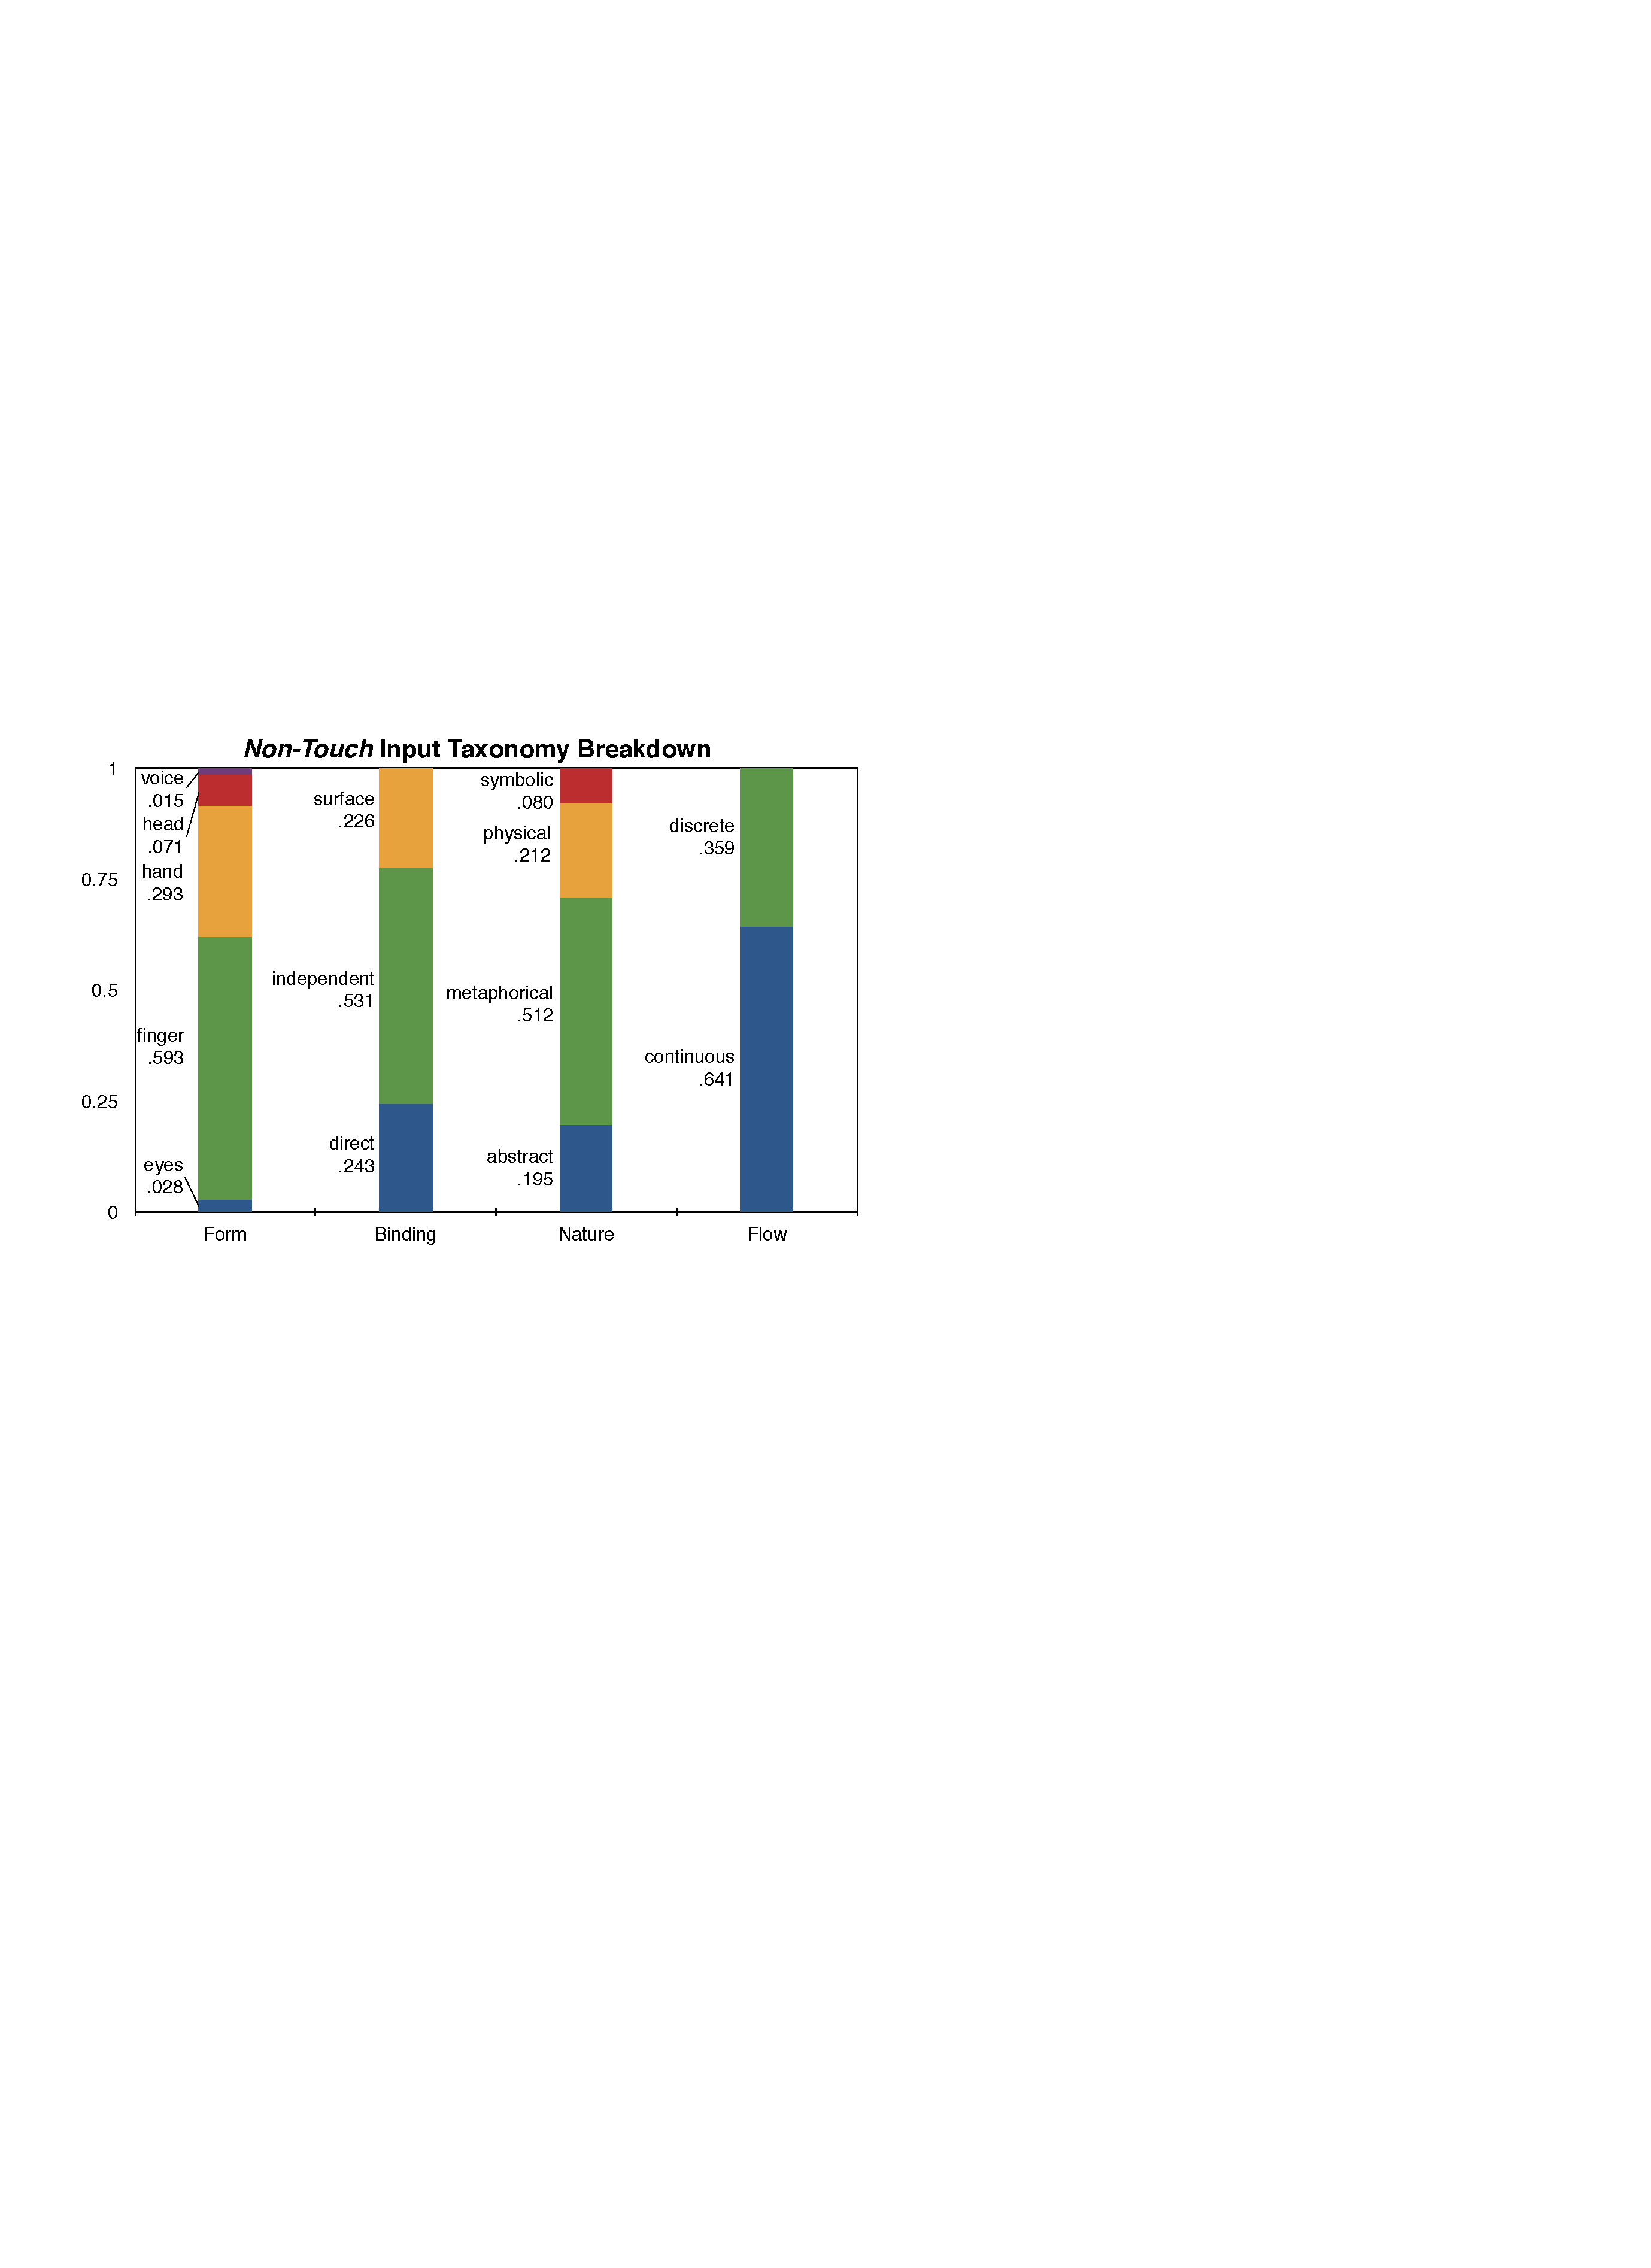
\includegraphics[width=1\columnwidth]{InAirTaxonomy.pdf}
  \caption{Percentage of game controls in each taxonomy category with in-air gesture.}
  \label{fig:InAirTaxonomy}
  \end{figure} 

 \begin{figure}[!h]
  \centering
  \includegraphics[width=1\columnwidth]{OnbodyTaxonomy.pdf}
  \caption{Percentage of game controls in each taxonomy category with on-body input.}
  \label{fig:OnbodyTaxonomy}
  \end{figure} 

  \subsection{User-Defined Game Control Set}
  At the heart of this work is the creation of a user-defined game control set with smart glasses in public space. This section gives the process by which the set was created and properties of the set. Unlike prior game control sets in traditional game platforms, this set is based on observed user behavior and joins user action to game tasks.

   \subsubsection{Agreement}
   After all 24 participants had provided game control for each game tasks with each glasses form and interaction methods, we grouped the game control within each task such that each group held identical controls. Group size was then used to compute an \emph{Agreement Scrore} that reflects, in a single number, the degree of consensus among participants. A task with .31 agreement score means that, random two users will has 31\% chance to perform the identical control action for this task. (The definition and formula of agreement score were refer to previous work \cite{Wobbrock:2005:MGS:1056808.1057043}.)
   \begin{equation}
   A = \frac{\displaystyle{\sum_{t\epsilon T }} \sum_{P_i \subseteq P_t } \left(\frac{\lvert{P_i}\rvert}{\lvert{P_t}\rvert}\right) ^ 2}{\displaystyle{\lvert{T}\rvert}}
   \end{equation}
  
   In eq. 1, $t$ is a task in the set of all tasks $T$, $P_{t}$ is the set of proposed control actions for task $t$, and $P_i$ is a subset of identical control action from $P_{t}$. The range for $A$ is $\left[\lvert{P_t}\rvert ^{-1}, 1\right]$. As an example, consider agreement for \emph{draw a path} with on-body input, it had four groups of identical control actions with groups size 34, 4, 5 and 5. we compute

   \begin{equation}
   A_{body-path} = \left(\frac{34}{48}\right) ^ 2  + \left(\frac{4}{48}\right) ^ 2 + \left(\frac{5}{48}\right) ^ 2 + \left(\frac{5}{48}\right) ^ 2 = 0.53
   \end{equation}

 Agreement for our study is graphed in Figure \ref{fig:Agreement}. The overall agreement for in-air and on-body inputs were $A_{Air}$=0.27 and $A_{Body}$=0.25, respectively. In comparison to the agreement of in-air and on-body inputs, we found their patterns were extreme similar. The average difference of agreement between these two interaction methods was .056. It implied that the agreement score was influenced more by the game tasks than by the interaction methods.


 \begin{figure}[!h]
  \centering
  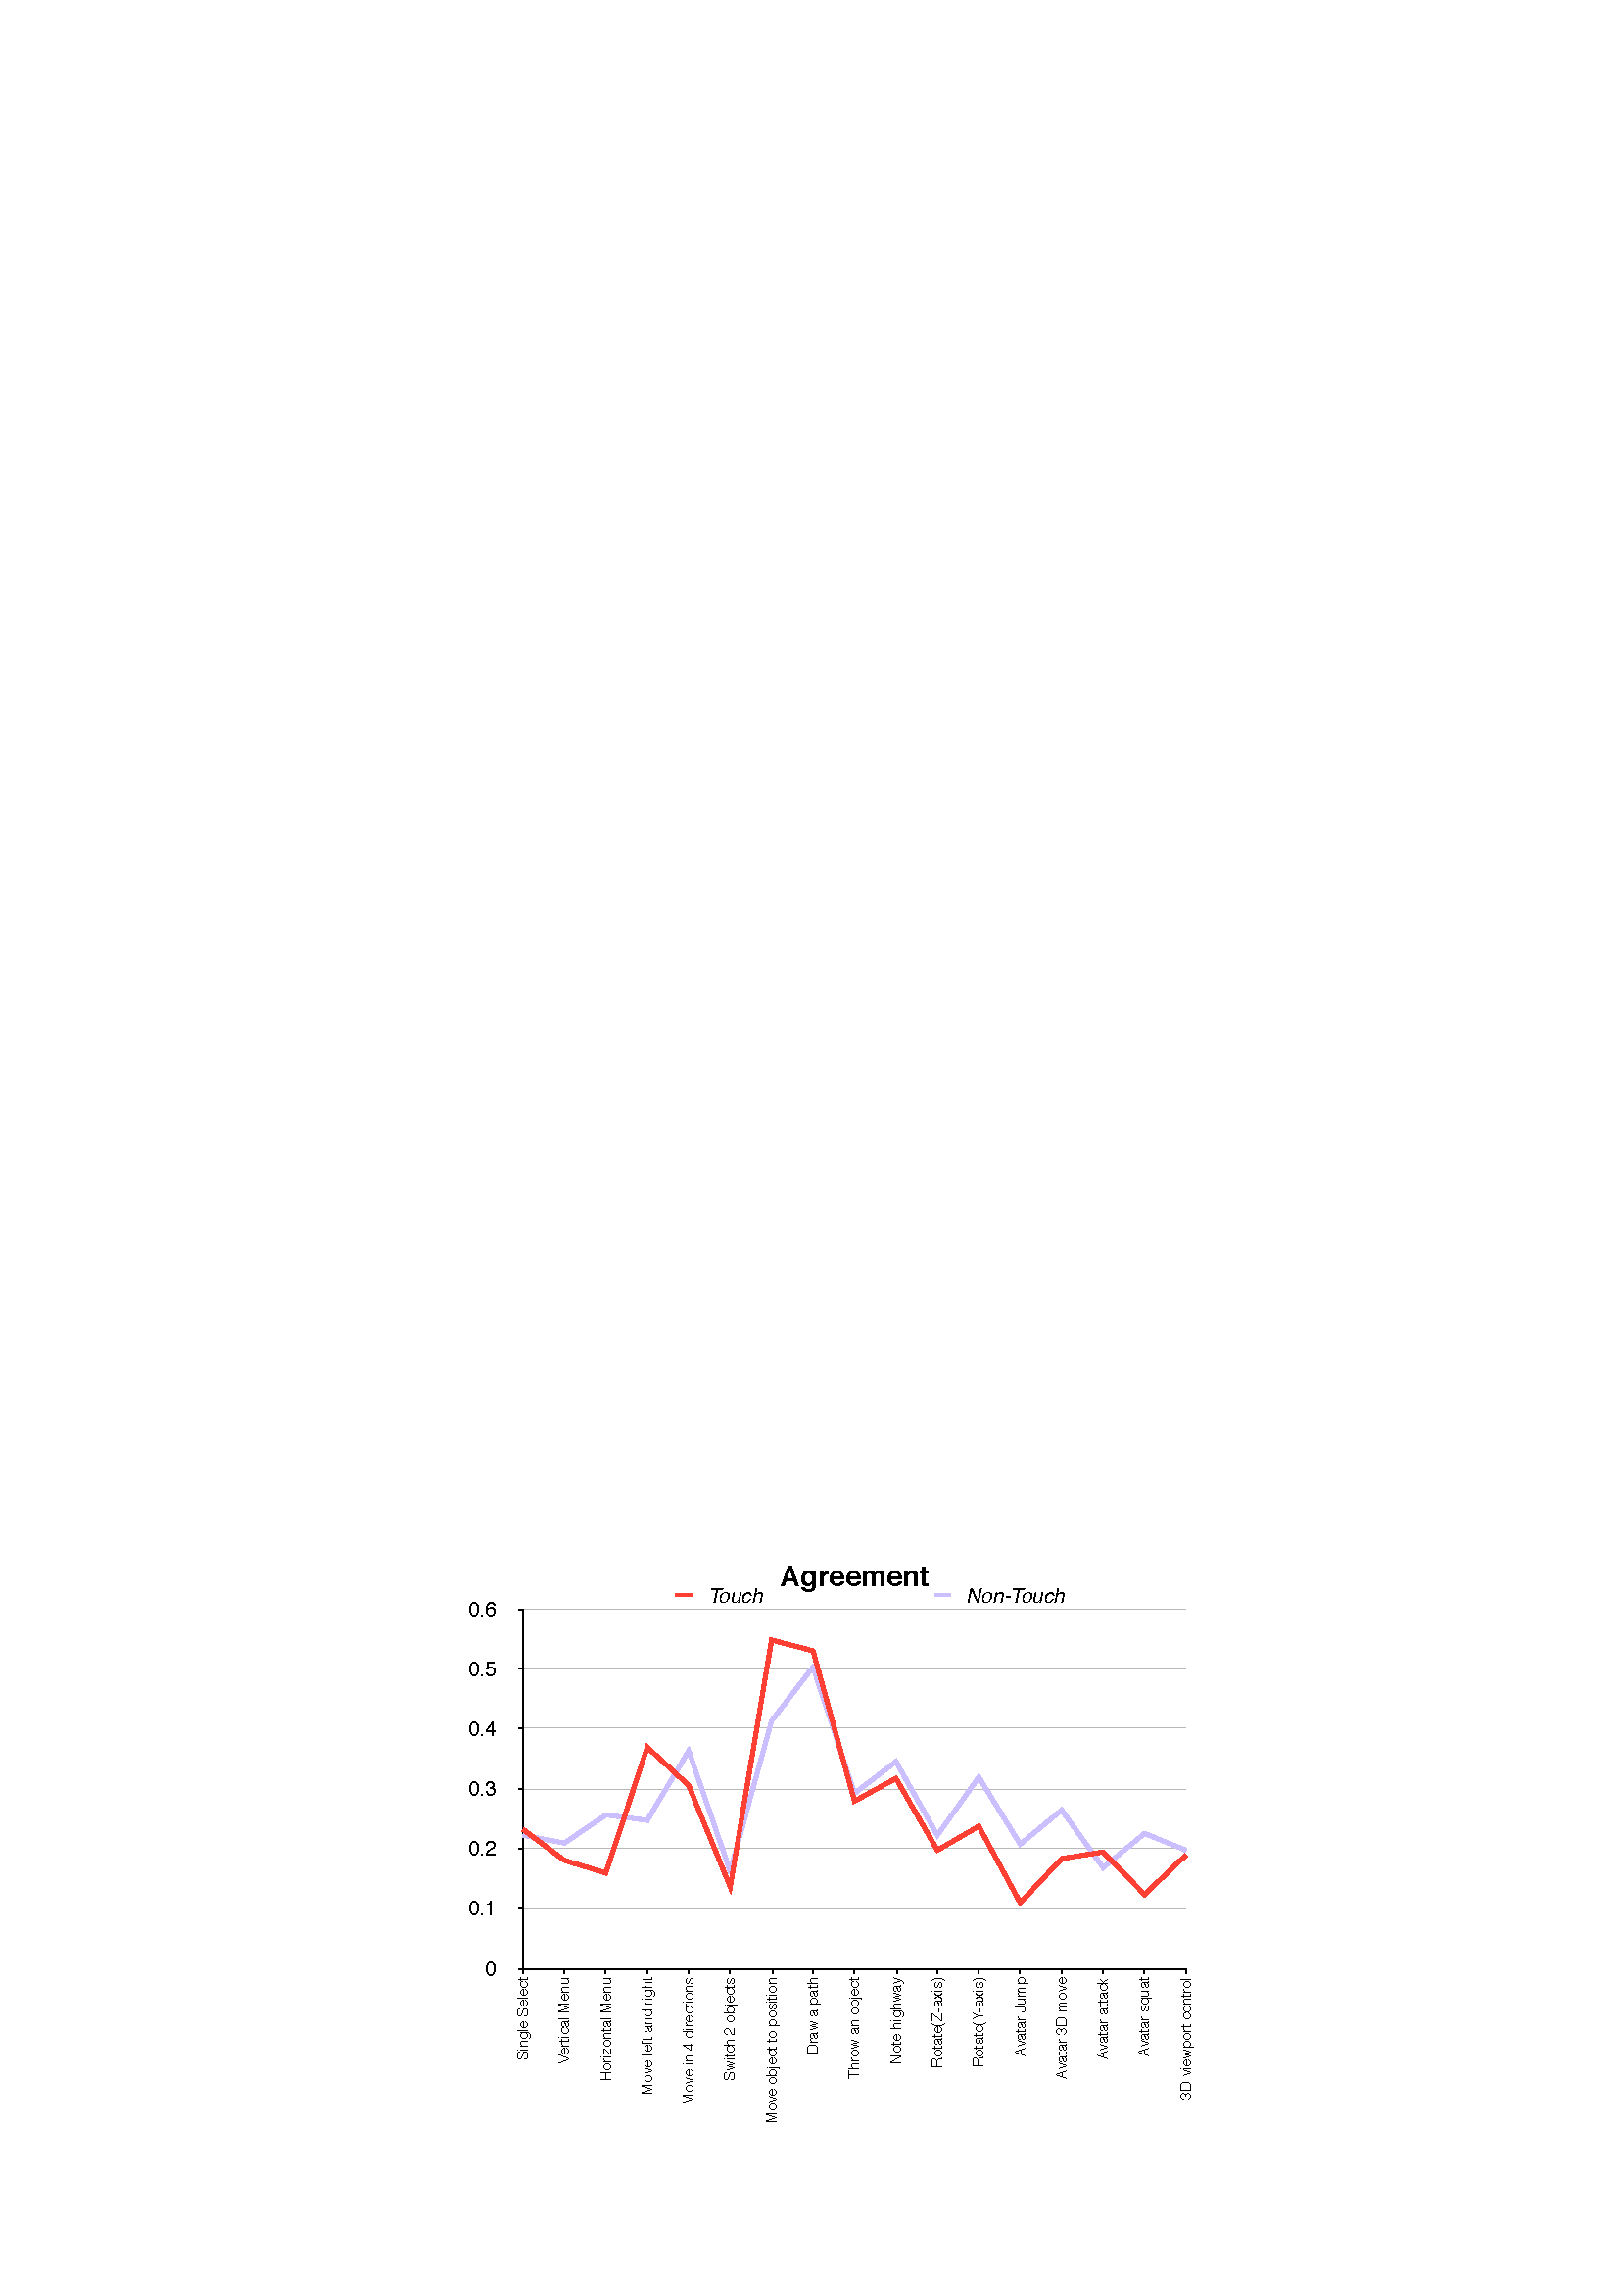
\includegraphics[width=1\columnwidth]{Agreement.pdf}

  \caption{Agreement for each game tasks. The tasks are listed in the same order as they appear in Table \ref{tab:table1}.}
  \label{fig:Agreement}
  \end{figure} 

   %\subsubsection{Conflict and Coverage}

   %Howerver, where the same control action was used to perform different game tasks, a conflict occurred if the game consists the tasks at same time. In our case ,we found that ``Move in 4 Directions'',``Avatar 3D Move'' and ``Viewport Controls'' are assigned with same control action with on-body input(Fig?.?). According to the property of our top 90 casual games, the average task count for these game is 2.56 (std=1.07). In another word, there are about 1 to 4 game tasks in each game title. There is a low chance to perform these three game controls at same game and same time. To make our game control set reflects more consistent with user behavior, we decide to remain it conflict. 


   \subsubsection{Properties of the User-defined Game Control Sets}
   The user-defined game control set was developed by taking largest groups with identical control for each game task and then assigned those groups' control to the task. 
   Our results of the user-defined game control set covered game controls with in-air gesture and on-body input with 40.07\% and 41.32\% respectively. Our user defined set is useful, therefore, not just for what it contains, but also for what it omits.

   With in-air gestures(see Figure \ref{fig:InAirSet} although we informed users to perform game control not limited with hands in advance, the result showed that users still preferred to use hand gestures rather than use voice controls, eye gesture and head tilting. Additionally, users would make use of direct-control if they had to perform precise task, such as selecting an object from many or moving an object to the specific position.As other tasks with lower precision requirement, such as selecting a single option from 4 or enabing an avatar jump. Users would prefer using an in-direct control. For example, users tapped 4 different area in front of their chest or raised hands slightly.


    All the controls in our final on-body input set are finger related (see Figure \ref{fig:OnBodyInputSet}). Most of them use single finger tip to perform gestures on different surfaces. And the most preferable surface for on-body gestures is hand palm. These controls seem like an trackpad or a proxy touch-screen. The remained controls are finger interaction with single hand. Specifically, users use thumb to interact with index finger or ring.

   \subsubsection{Taxonometric Breakdown of User-Defined Game Controls}
   As we should expect, the taxonometric breakdown of the final user-defined game control sets(Figure \ref{fig:InAirSet} and \ref{fig:OnBodyInputSet}) are similar to the proportions of all control actions proposed (Figure \ref{fig:InAirTaxonomy} and \ref{fig:OnbodyTaxonomy}). Across all taxonomy categories, the average difference between these two sets were only 3.09\% and 6.31\% respectively.

  \subsection{Mental Model Observations}
    \subsubsection{Social Acceptance and Control Area}
    To our surpirsed, approximately 63\% of in-air ``hand'' user-defined gestures were not performed in front of their face (See Figure.\ref{fig:figureInAirPorpotion}.E). This behavior conflicted with current ``Google Glass'' design and previous works\cite{Colaco:2013:MCL:2501988.2502042}. There were 7 participants perfoming more gestures in front of face than other position. They indicated that control in front of face was more precise and intuitive. At the same time, the other 17 users preferred to perform in-air gesture in front of their chest or below. Among them, there are 3 participants never performed any in-air gesture in front of their face. These users indicated that moving a finger in front of their face was really weird and not social acceptable. And there was also a hand strained problem to lift hand in front of face. They thought it was not suitable for game control.

    \subsubsection{Metaphor from Exisiting Game Control}
    Although we took care not to show elements from traditional game platforms like Consoles, PCs or Mobile games, participants still often thought with the previous gaming experience. For example, some controls actions performed as if using touch-screen in front of their face (see Figure.\ref{fig:InAirSet}.A,F,G). And some actions is similiar with using a imaginary trackpad on in-air surface or hand surface(see Figure \ref{fig:InAirSet}.\{H,I\} and Figure \ref{fig:OnBodyInputSet}.\{B,D,E,F,G,J,K,M\}). Moreover, an imaginary button on the index finger(Figure \ref{fig:OnBodyInputSet}.Q). Even with simple shapes and basic character, it was clear how deeply rooted the previous gaming experience is. Some quotes reveal this: ``just click the button like a joystick,''``can I just image there is a trackpad on my palm?''``It's a imaginary touch-screen.''

\subsubsection{Identical Gestures on Different Surfaces}
 In our study, we found several identical gestures performed by our users with different surfaces. Take the task ``Move in 4 directions'' for example, although 57\% of gestures were performed by moving finger on the palm with on-body inputs(Figure \ref{fig:OnBodyInputSet}.E). The rest gestures were mostly using identical gestures on the different surfaces such as handback, leg, forearm and even face. Same phenomena could also be observed by comparing the game control between our two user-defined game control sets. ``Move left and right'', ``Move in 4 directions'', ``Draw a Path'', ``Throw an Object'' were assigned with identical gestures with palm surfaces and in-air imaginary surfaces (See Figure \ref{fig:InAirSet}\{D,E,H,I\} and Figure \ref{fig:OnBodyInputSet}\{D,E,J,K\}). In these cases, the surfaces did not influence the meaning of gestures, which could be performed on any surfaces. We have asked users why they choosed palm as their input area. The general response was concerning about the lowest physical movement demand, such as ``I choose left palm to perform gesture because it is near to my right index finger''.


  \begin{figure*}
  \centering
  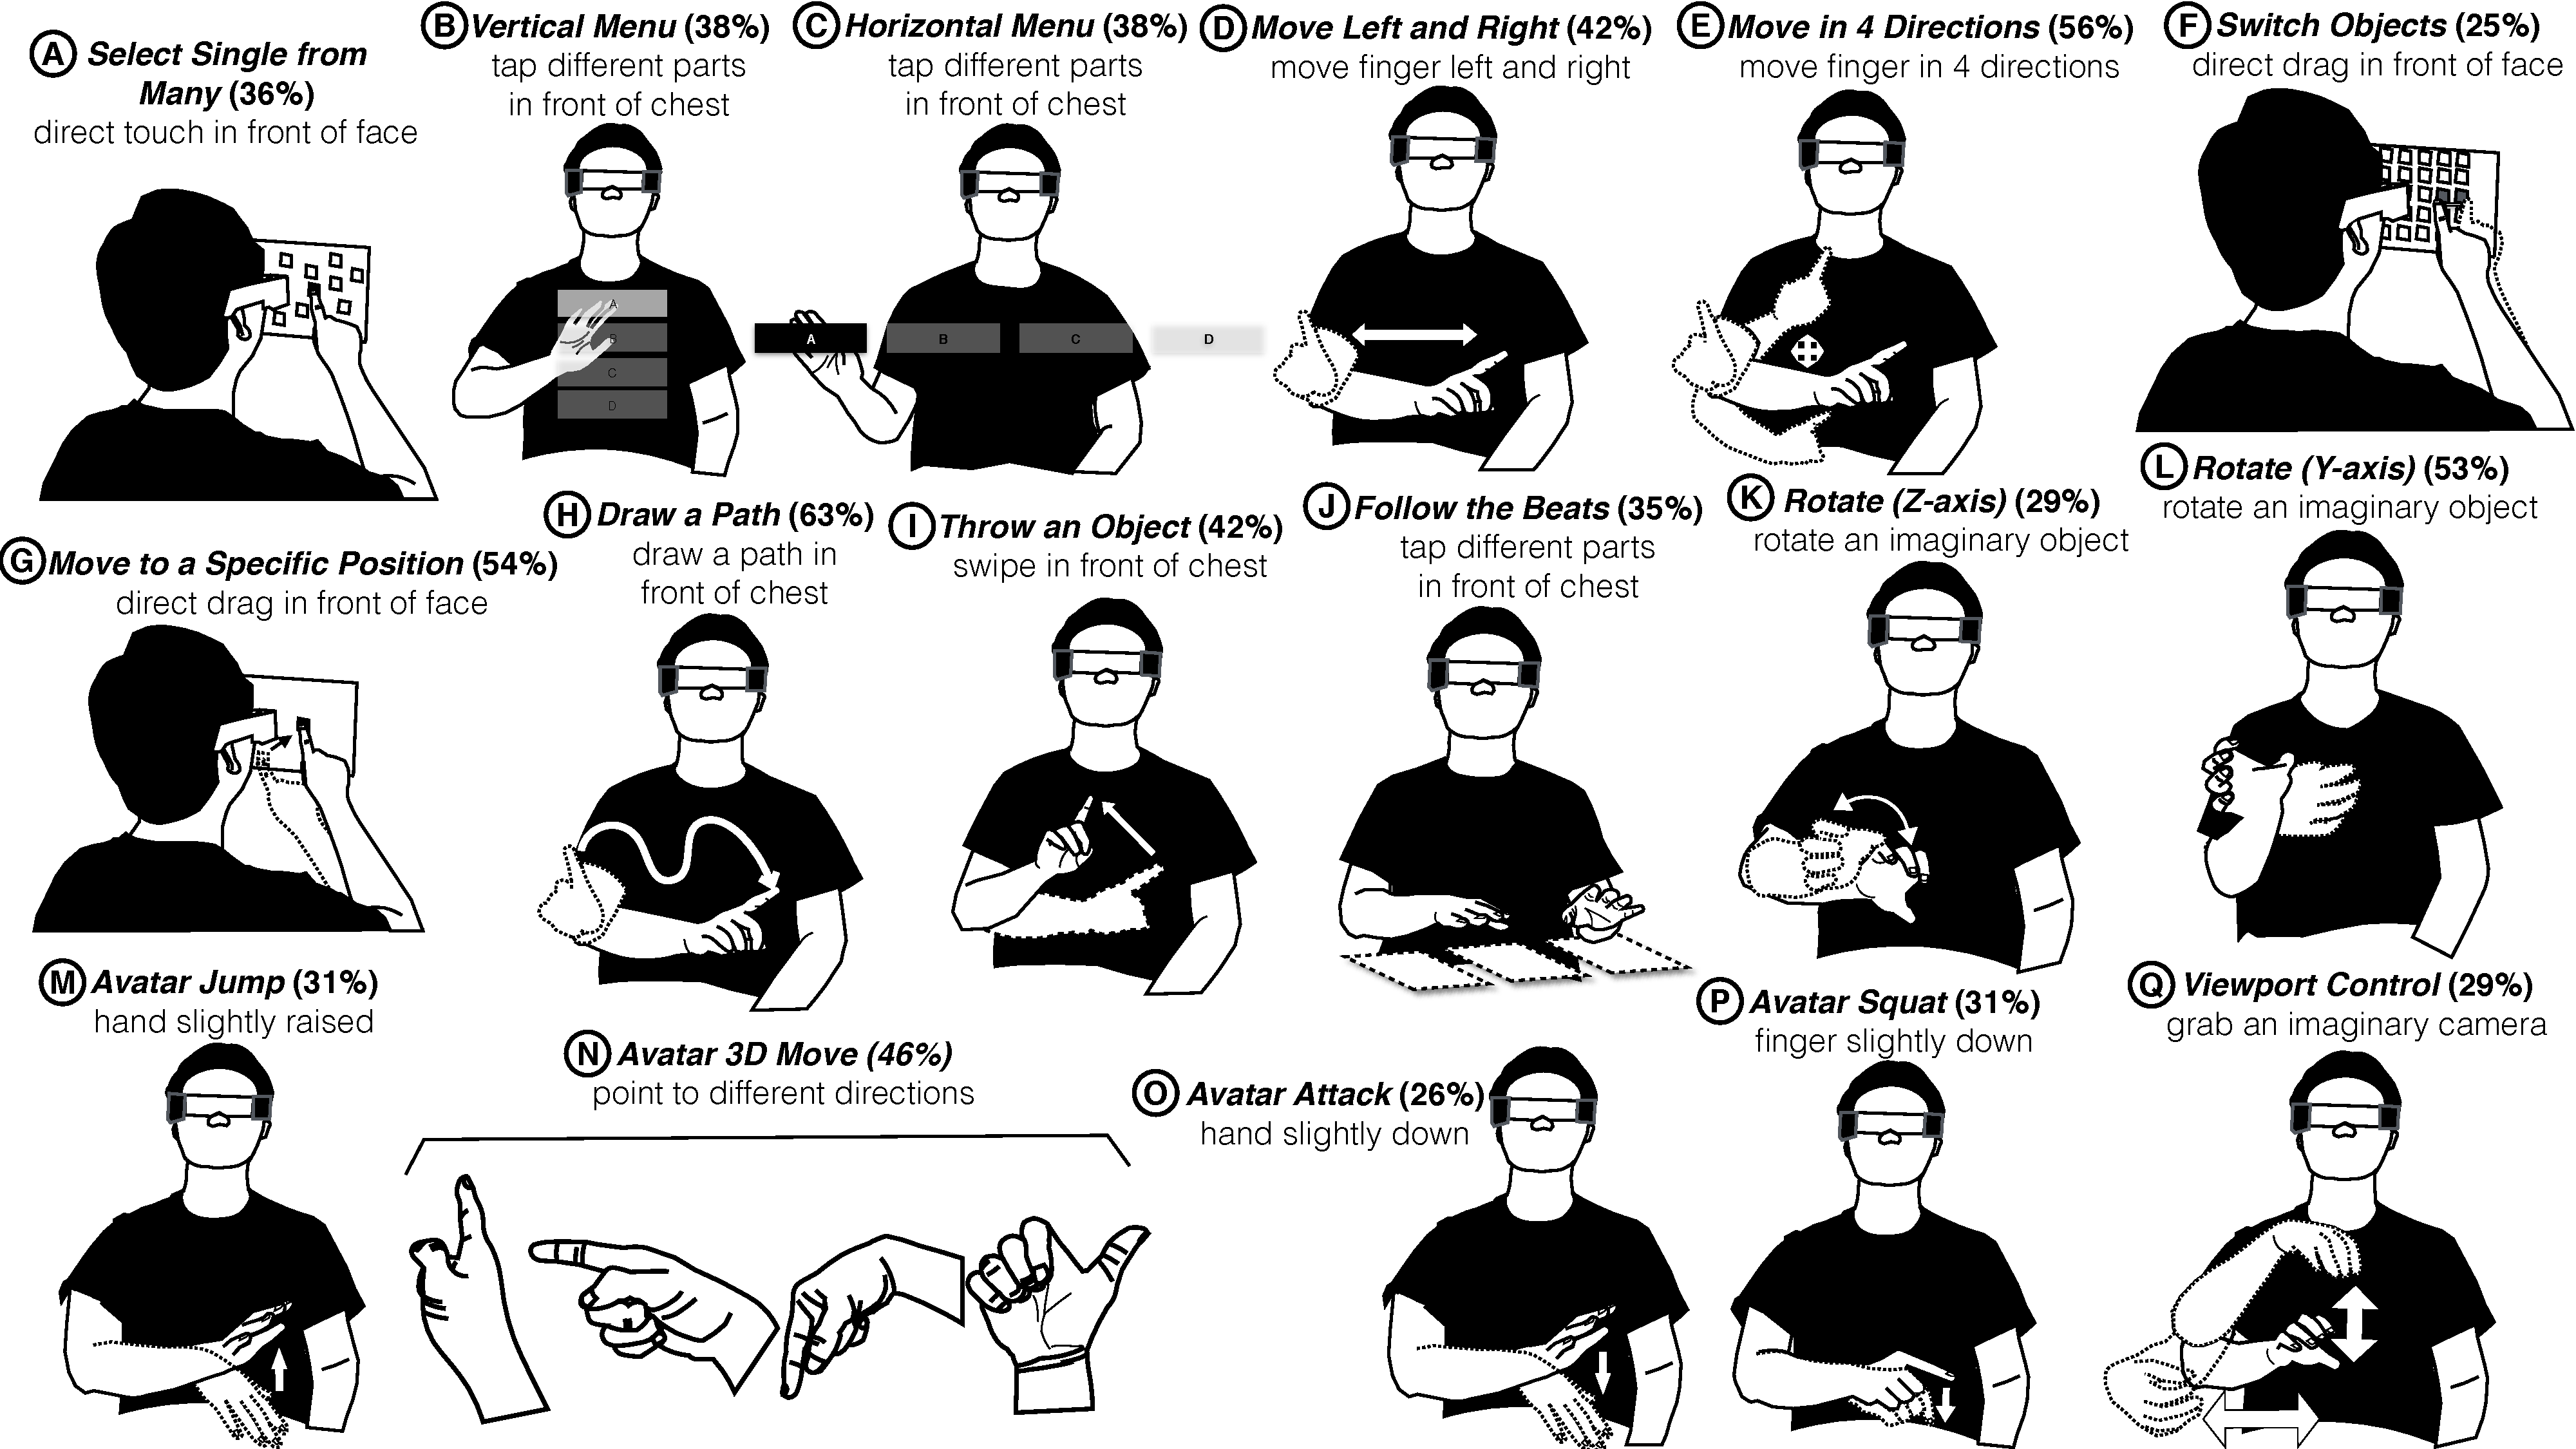
\includegraphics[width=1\textwidth]{InAirSet.pdf}
  \caption{The user-defined game control set with in-air gesture, The percentage indicate the portion of users who perform the control action for the game task.}
  \label{fig:InAirSet}
  \end{figure*}


  \begin{figure*}
  \centering
  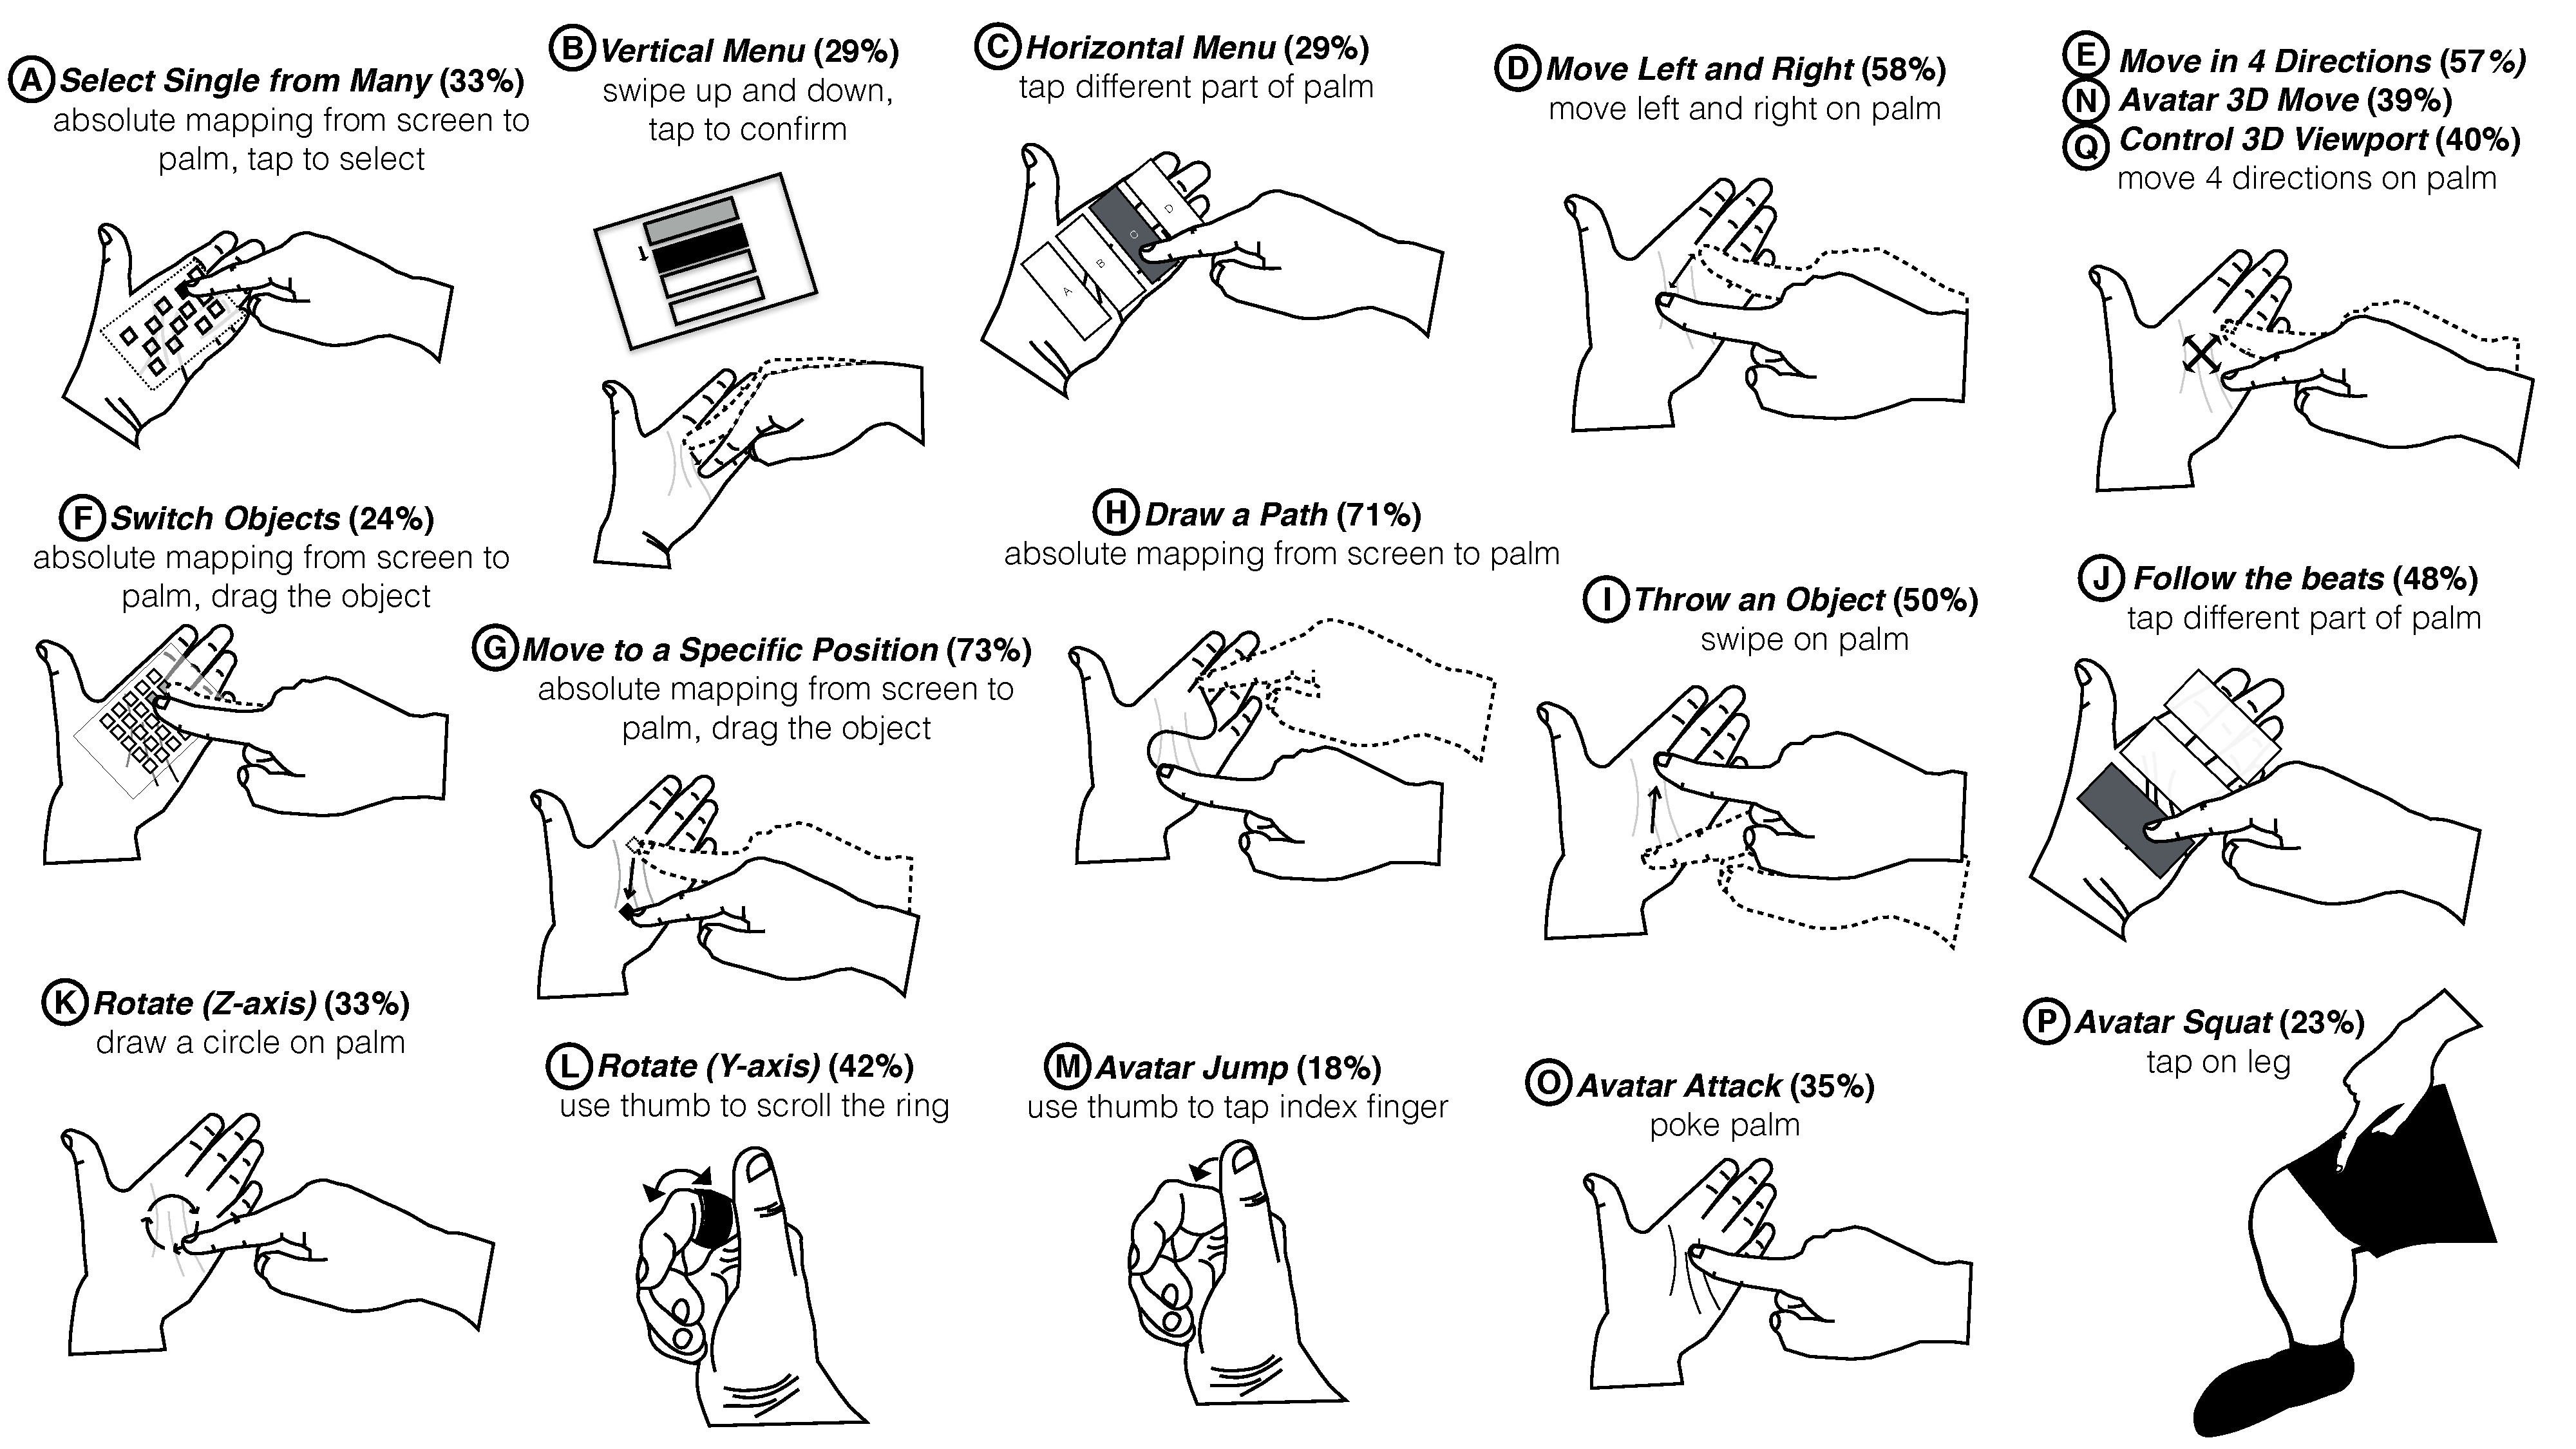
\includegraphics[width=1\textwidth]{OnBodyInputSet.pdf}
  \caption{The user-defined game control set with on-body inputs. The percentage indicate the portion of users who perform the control action for the game task. Note that, there are 3 tasks (``Move in 4 directions'',``Avatar 3D Move'',``Viewport Control'') have been assigned with an identical control action.}
  \label{fig:OnBodyInputSet}
  \end{figure*}


  \section{Discussion}
    %\subsubsection{Users' and Designers' Gestures}
    \subsubsection{Implications for In-Air Gesture Technology}
    With in-air interaction methods, our taxonomy shows that finger and hand are still the dominant  forms for smart glass gaming (Figure \ref{fig:figureInAirPorpotion}.{A,B}). there are only a small number to use head-gesture, eye-gesture and voice controls, 7\%, 3\% and 1\% respetively.
    Before the study began, both Google Glass and Epson\cite{GoogleGlass, Colaco:2013:MCL:2501988.2502042} supplied their own in-air gesture sets to increase the diversity of their input. However, the result showed that 63\% in-air gestures were not performed in front of users' faces in the public space due to social acceptance and physical tiring issues metioned by feedback (see Figure \ref{fig:figureInAirPorpotion}.E). Therefore, if the developers of head worn devices want to implement in-air gestures for input, they will need to have the capablity for sensing gestures in a wide range of areas near users. Take CV-based sensing technologies for example, they can use wide-angle lens or fish-eye lens to carry out a gesture set in order to cater to users' preference.   
  \begin{figure}[!h]
  \centering
  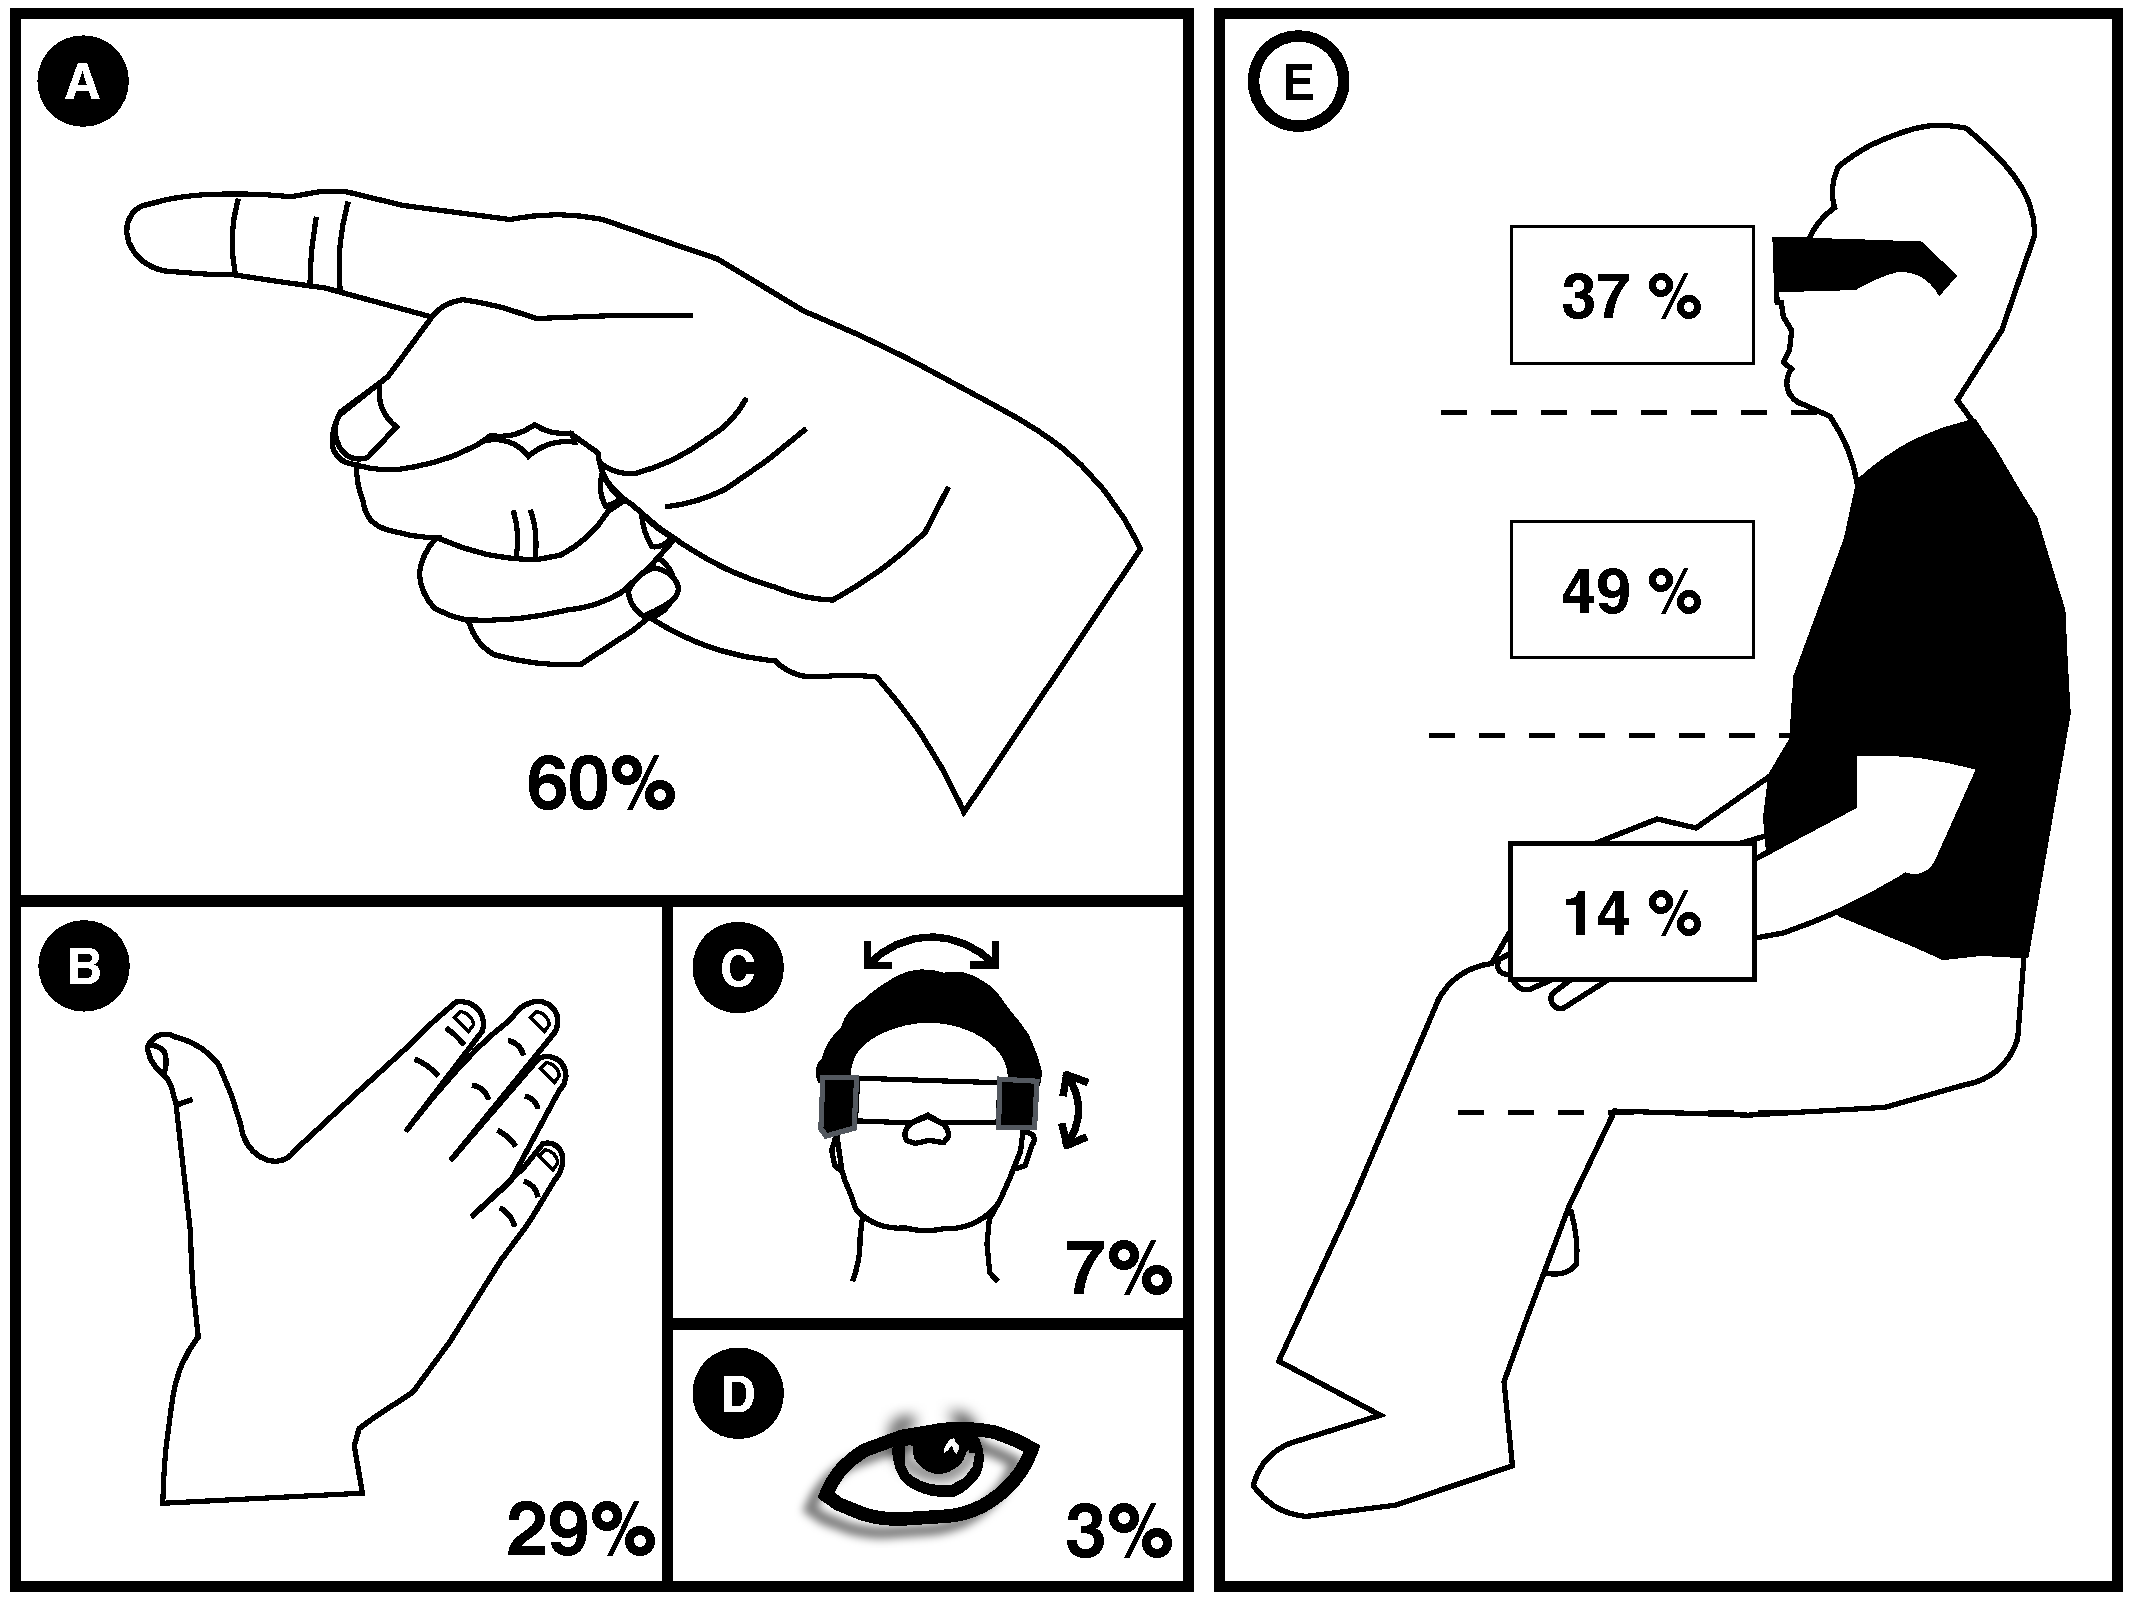
\includegraphics[width=1\columnwidth]{InAirControlArea.pdf}
  \caption{Form summary of in-air gesture. (A)Using finger to perform in-air gesture. (B)Using full hand to perform in-air gesture. (C)Using head-tilting or rotating to perform game control. (D)Perfrom game control with eyes-gesture. (E)The portion of in-air ``hand'' gesture control area. Half of in-air gestures (49\%) were performed in front of their chest, 14\% were in front of belly or below. Only 37\% gestures were performed in front of their face.}
  \label{fig:figureInAirPorpotion}
  \end{figure}
  \subsubsection{Implications for On-Body Input Technology}
    Our results showed that palm was the most favorite area for users to perform on-body inputs. Half of the game controls with on-body input used a finger to perform gesture on palm (See Figure \ref{fig:figureOnBodyPorpotion}). According to the mental model mentioned above, users utilized the metaphor of trackpad and touch-screen on the palm in several cases. Current gesture-recognizer on trackpad and touch-screen might be a suitible implementation reference for these input controls.

    From another point of view, all these controls were conducted by fingers of users dominant hand. If possible, we suggested that the sensing area should be targeted around the dominant hand finger rather than other specific parts of body, such as palm or leg. Hence, you could sense almost all cases of users' on-body inputs. Take CV-based sensing techonologies for example, we should put the fish-eye lens around the dominant hand finger rather than palm.

  \subsubsection{Implications for Game Design}
  According to the agreement scores we found, no matter using in-air gesture or on-body input, the average agreement between users were only .26, and the highest one was just about .55 (see Figure \ref{fig:Agreement}). In this case, guessing the game control would become a frustrating experience for users. It indicated that game developers should design the visual guide carefully to lead users performimg the control action, or show a helping instruction to explain the control methods.


 \begin{figure}[!h]
  \centering
  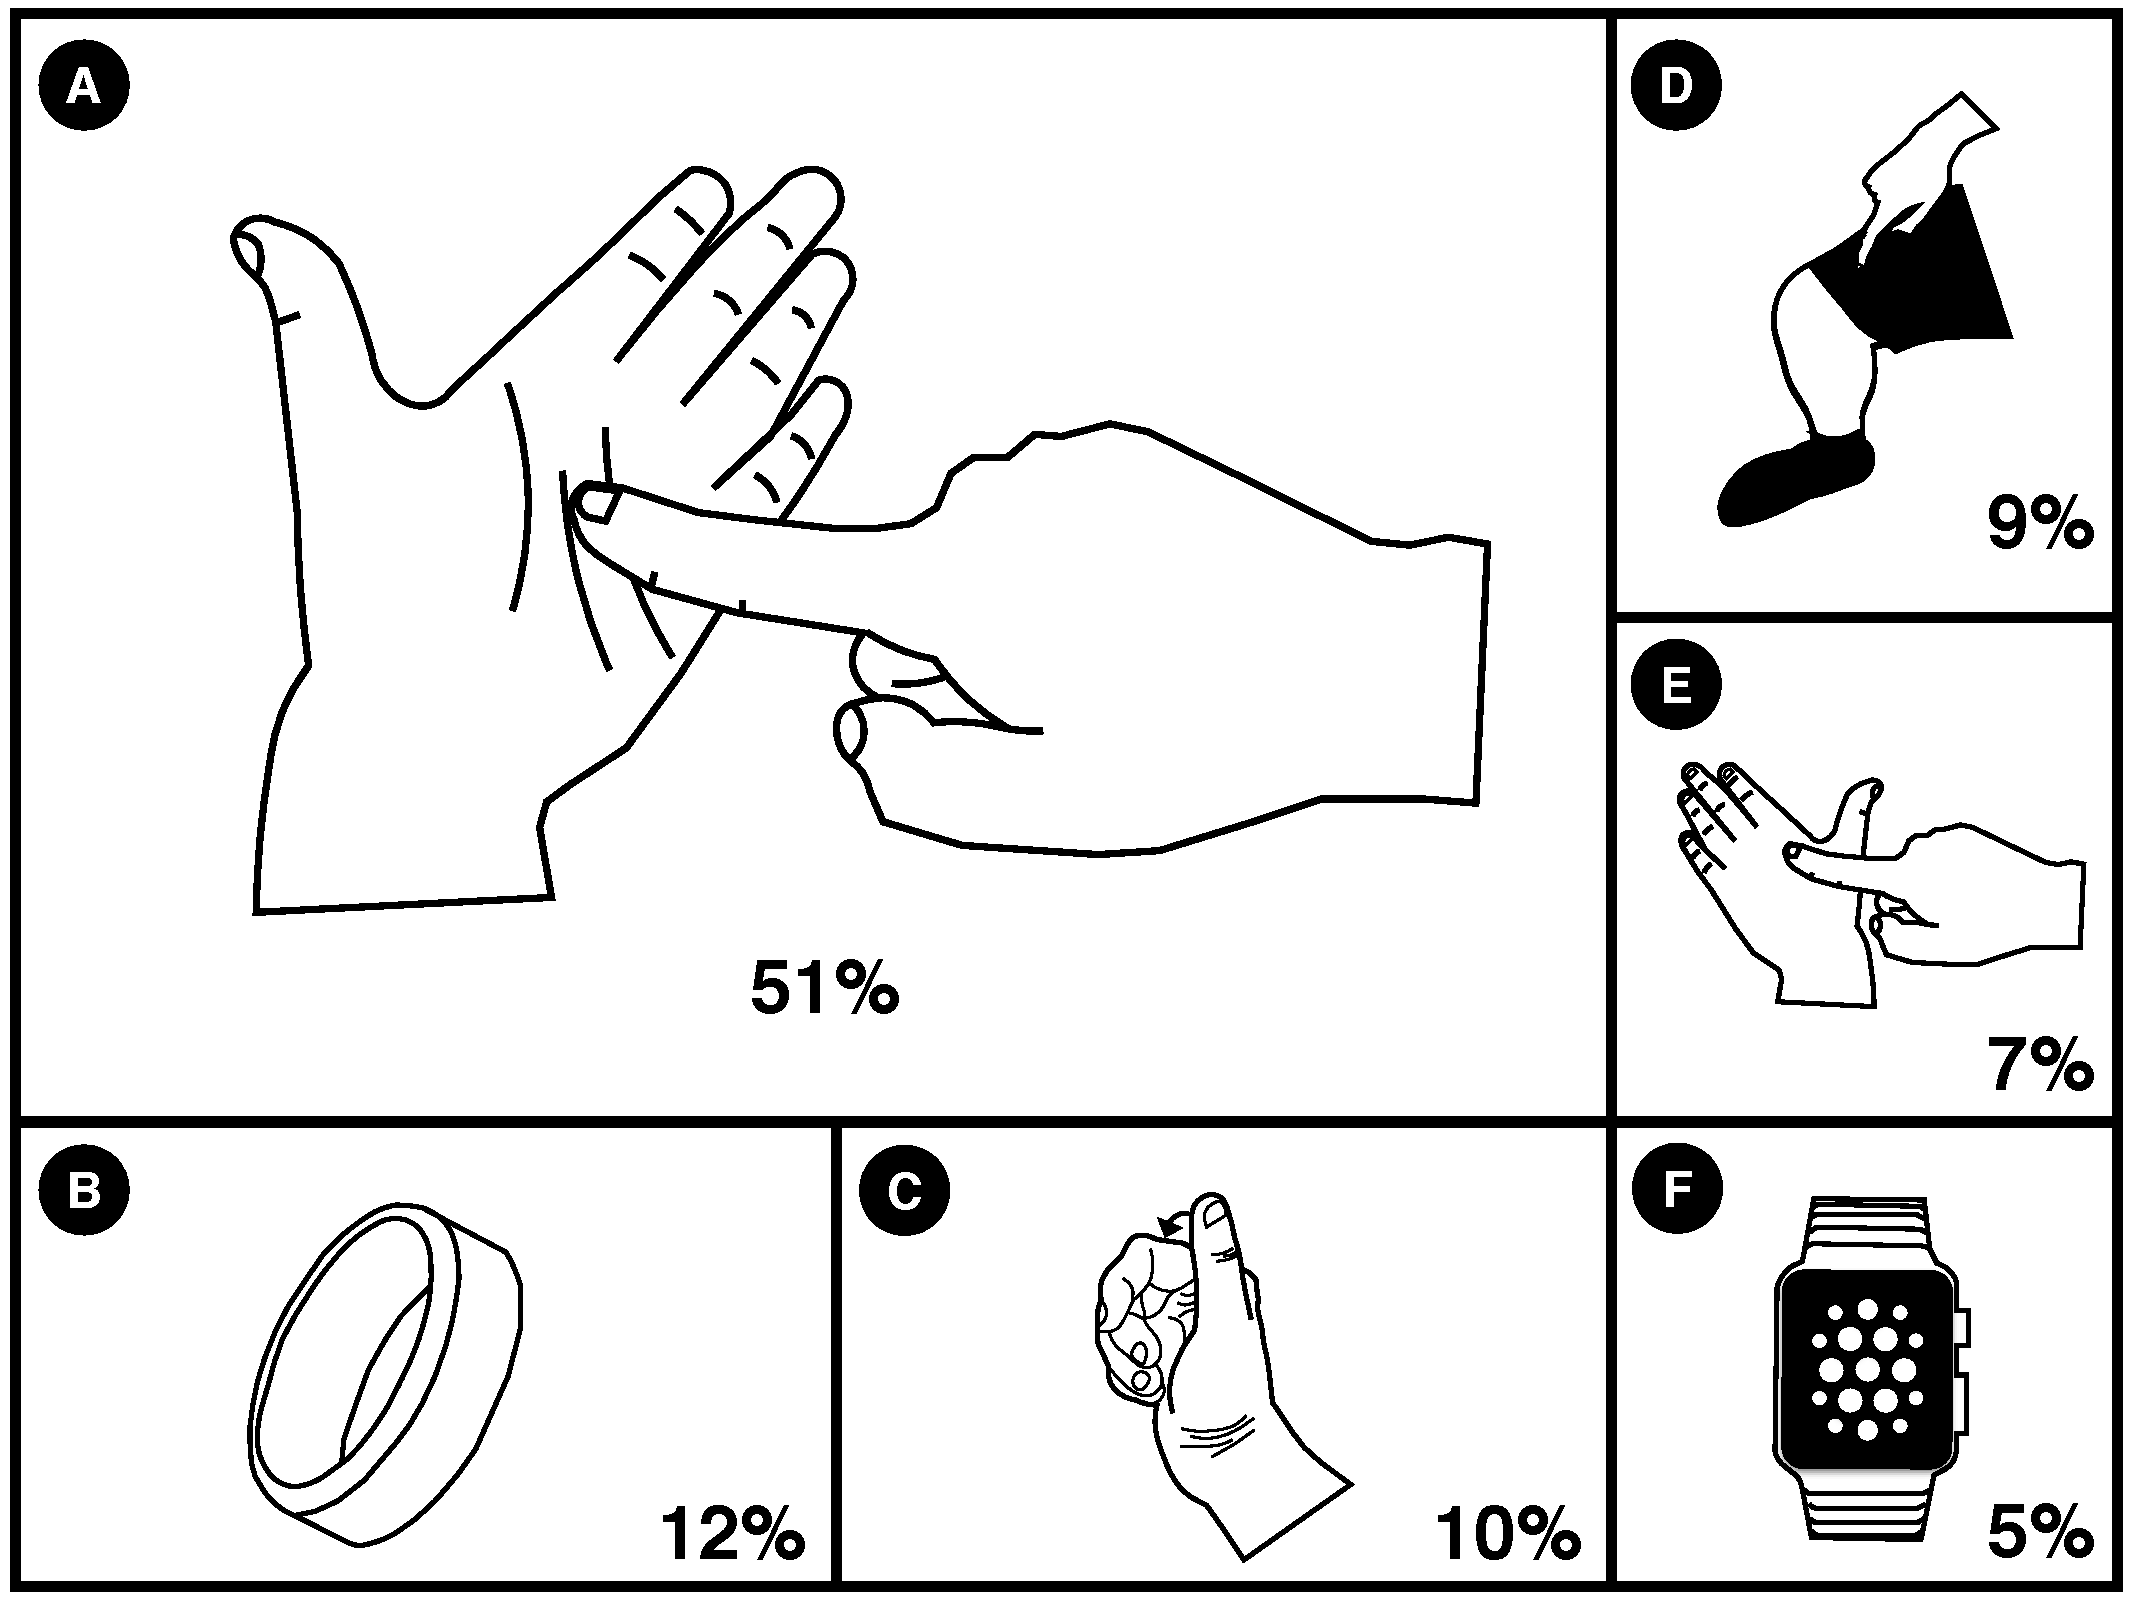
\includegraphics[width=1\columnwidth]{OnBodyForms.pdf}
  \caption{The top 6 on-body input forms. Percentages indicate the portion of game controls were performed. (A)Interact between finger and palm. (B)Interact with ring. (C)Interact between fingers.(D)Interact between finger and leg. (E)Interact between finger and hand back. (F)Interact with watch.}
  \label{fig:figureOnBodyPorpotion}
  \end{figure}   

  %\subsubsection{Implications for User Interfaces}
  \subsubsection{Limitation and Next Steps}

  In our work, we showed the single game task independent to users. Users designed these controls without the overview of all tasks. Our resulting sets might conflicted with each other if we wanted to perform two or three controls simultaneously. For example, with on-body input, users would feel unconfortable to move in 4 directions and performed avatar attack at the same time (see Figure \ref{fig:OnBodyInputSet}\{F,N\}). In future work, we will try more possibility to show users the combination of multiple tasks and to understand more about how users behavior alternation under this circumstance.

  As we know, there are many places known as public space, and users may behave differently in each place. Futhermore, in our study, we did not ask users to define any control actions to interact with tangible objects in public space, such as, tables or chairs in the cafe. We only requested participants to experience two types of Smart Glasses. Therefore, our user-defined game control sets might not suit to be applied to games on other types of head worn devices. Moreover, our participants were all literate Taiwanese adults; Undoubtedly, childern, elders, Westerners, or uneducated participants would behave differently. That is to say, these issues are worthy of investigation, but exceed the range of our current work.

  An important next step is to validate our user-defined game control set with a wearable system, which can sense all in-air and on-body control actions listed in our set.   
    %Glass Forms 只有兩種
    %Culture問題?
    %Interaction with 桌椅?


\section{Conclusion}

We have presented a user-defined game control set by performing a study of glass game control with participants' agreement over 2448 gestures.
It can reflect the user gaming behavior and habit in public space, such as choosing a relatively unobtrusive area to perform game control. In addition, We firmly believe that our user defined game control set is also a good candidate for development in glass game control system. In other words, we have presented a taxonomy of glass game controls for analyzing and characterizing control actions with smart glasses. 
In capturing game controls for this study, we have gained insight into the mental models of public users and have tranlated these into implications for techonoloy and design. 
This work represents a necessary step in bringing smart glass gaming closer to the hands and minds of public people. And it also becomes a milestone to help designers create games on smart glasses for better users' experience.

%It is important that you write for the SIGCHI audience.  Please read
%previous years' Proceedings to understand the writing style and
%conventions that successful authors have used.  It is particularly
%important that you state clearly what you have done, not merely what
%you plan to do, and explain how your work is different from previously
%published work, i.e., what is the unique contribution that your work
%makes to the field?  Please consider what the reader will learn from
%your submission, and how they will find your work useful.  If you
%write with these questions in mind, your work is more likely to be
%successful, both in being accepted into the Conference, and in
%influencing the work of our field.

%\section{Acknowledgments}

%We thank CHI, PDC and CSCW volunteers, and all publications support
%and staff, who wrote and provided helpful comments on previous
%versions of this document.  Some of the references cited in this paper
%are included for illustrative purposes only.  \textbf{Don't forget
%to acknowledge funding sources as well}, so you don't wind up
%having to correct it later.

% Balancing columns in a ref list is a bit of a pain because you
% either use a hack like flushend or balance, or manually insert
% a column break.  http://www.tex.ac.uk/cgi-bin/texfaq2html?label=balance
% multicols doesn't work because we're already in two-column mode,
% and flushend isn't awesome, so I choose balance.  See this
% for more info: http://cs.brown.edu/system/software/latex/doc/balance.pdf
%
% Note that in a perfect world balance wants to be in the first
% column of the last page.
%
% If balance doesn't work for you, you can remove that and
% hard-code a column break into the bbl file right before you
% submit:
%
% http://stackoverflow.com/questions/2149854/how-to-manually-equalize-columns-
% in-an-ieee-paper-if-using-bibtex
%
% Or, just remove \balance and give up on balancing the last page.
%
\balance

%\section{References format}
%References must be the same font size as other body text.
% REFERENCES FORMAT
% References must be the same font size as other body text.

\bibliographystyle{acm-sigchi}
\bibliography{sample}
\end{document}
